\documentclass{ctexart}
\usepackage{amsmath}
\usepackage{float}
\usepackage{amssymb}
\usepackage{graphicx}
\usepackage{gbt7714}
\usepackage{pifont}
\usepackage{wrapfig}
\ctexset{
    % 修改 section。
    section={   
        name={,、},
        number={\chinese{section}}
    }
}

\title{RLC交流电路的稳态特性}
\author{陆知辰-10225301478}
\date{\today}
\graphicspath{{figure/}}

\begin{document}

\begin{titlepage}
  \centering
  % 插入图片
  
\includegraphics[width=0.5\textwidth]{ecnu.png}
  
  % 空行用于调整标题位置
  \vspace*{\baselineskip}
  
  % 标题
  \Huge\textbf{物\quad 理\quad 实\quad 验 \quad (二)}
  % 空行用于调整标题和其他信息之间的间距
  \vspace*{0.3\baselineskip}
  
  % 具体实验名称
  \huge RLC交流电路的稳态特性
  
  % 空行用于调整时间和其他信息之间的间距
  \vspace*{2\baselineskip}
  
  % 时间
  \large 时间:\today
  
  % 空行用于调整时间和其他信息之间的间距
  \vspace*{\baselineskip}
  
  % 创作人
  \large 创作人:陆知辰
  
  % 空行用于调整创作人和学号之间的间距
  \vspace*{\baselineskip}
  
  % 学号
  \large 学号:10225301478
  
\end{titlepage}
\newpage
\tableofcontents
\newpage
\section{实验摘要}
  \subsection{实验概要}
  电阻R,电感L和电容C是电路中最常见的三种元件。其中每个元件的作用如下:\newline
  电阻:限流作用,类似于接在两根大直径管子之间的小直径管子限制水流量的作用,也能保护电路。\newline
  电容:电容器是一种能够储藏电荷的电子元件。\newline
  电感:主要起到滤波、振荡、延迟、陷波等作用,还有筛选信号、过滤噪声、稳定电流及抑制电磁波干扰等作用。

  本实验研究RLC交流电路的稳态特征,并对RLC串联电路的品质因数Q进行测量

  \subsection{实验目的}
  1.\quad 研究RLC串联电路中电流和电源频率的关系。

  2.\quad 了解RLC串联谐振电路品质因数Q的物理意义,学习其测量方法。
  
  3.\quad 了解交流电路的连接要求,能够根据Q值的测量要求选择频率调节的范围。

\begin{figure}[H]
  \begin{minipage}[H]{0.4\textwidth}\label{rlcdianlu}
  \centering
  \caption{RLC电路}
  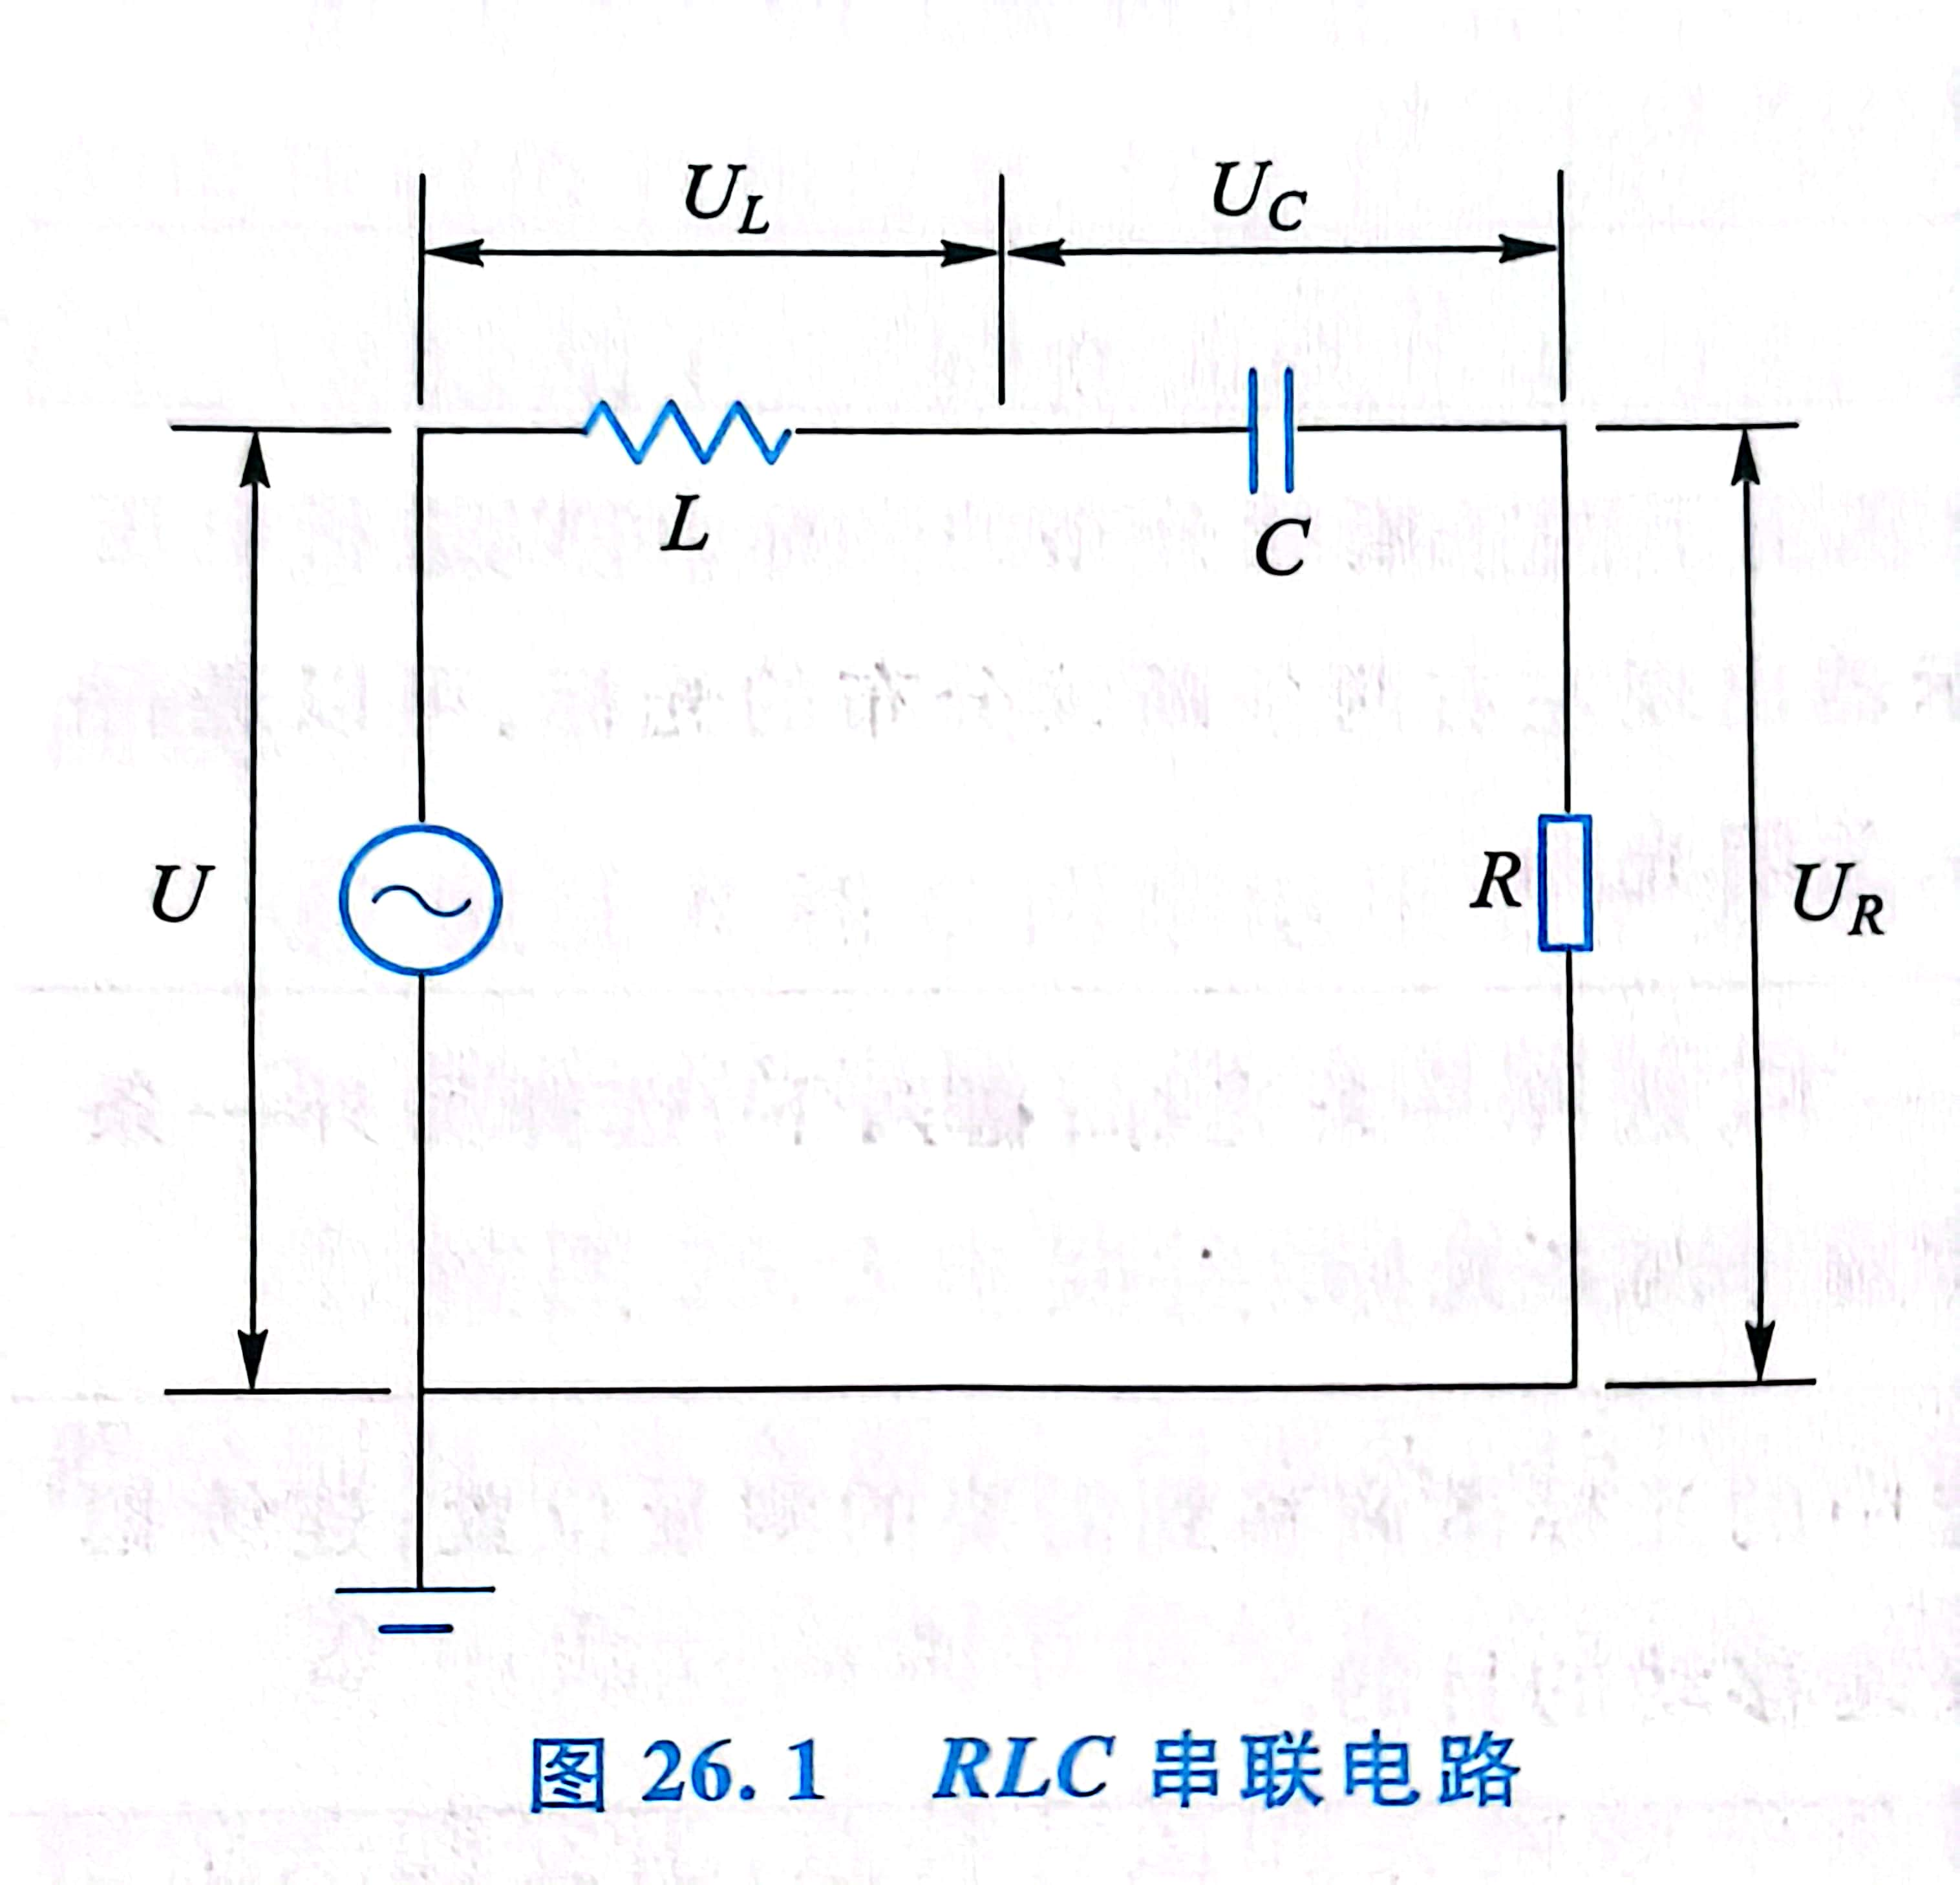
\includegraphics[width=\textwidth]{RLCdianlu.jpg}
  \end{minipage}
  \hfill
  \begin{minipage}[H]{0.4\textwidth}\label{rlcwentaitexing}
  \centering
  \caption{RLC稳态特性}
  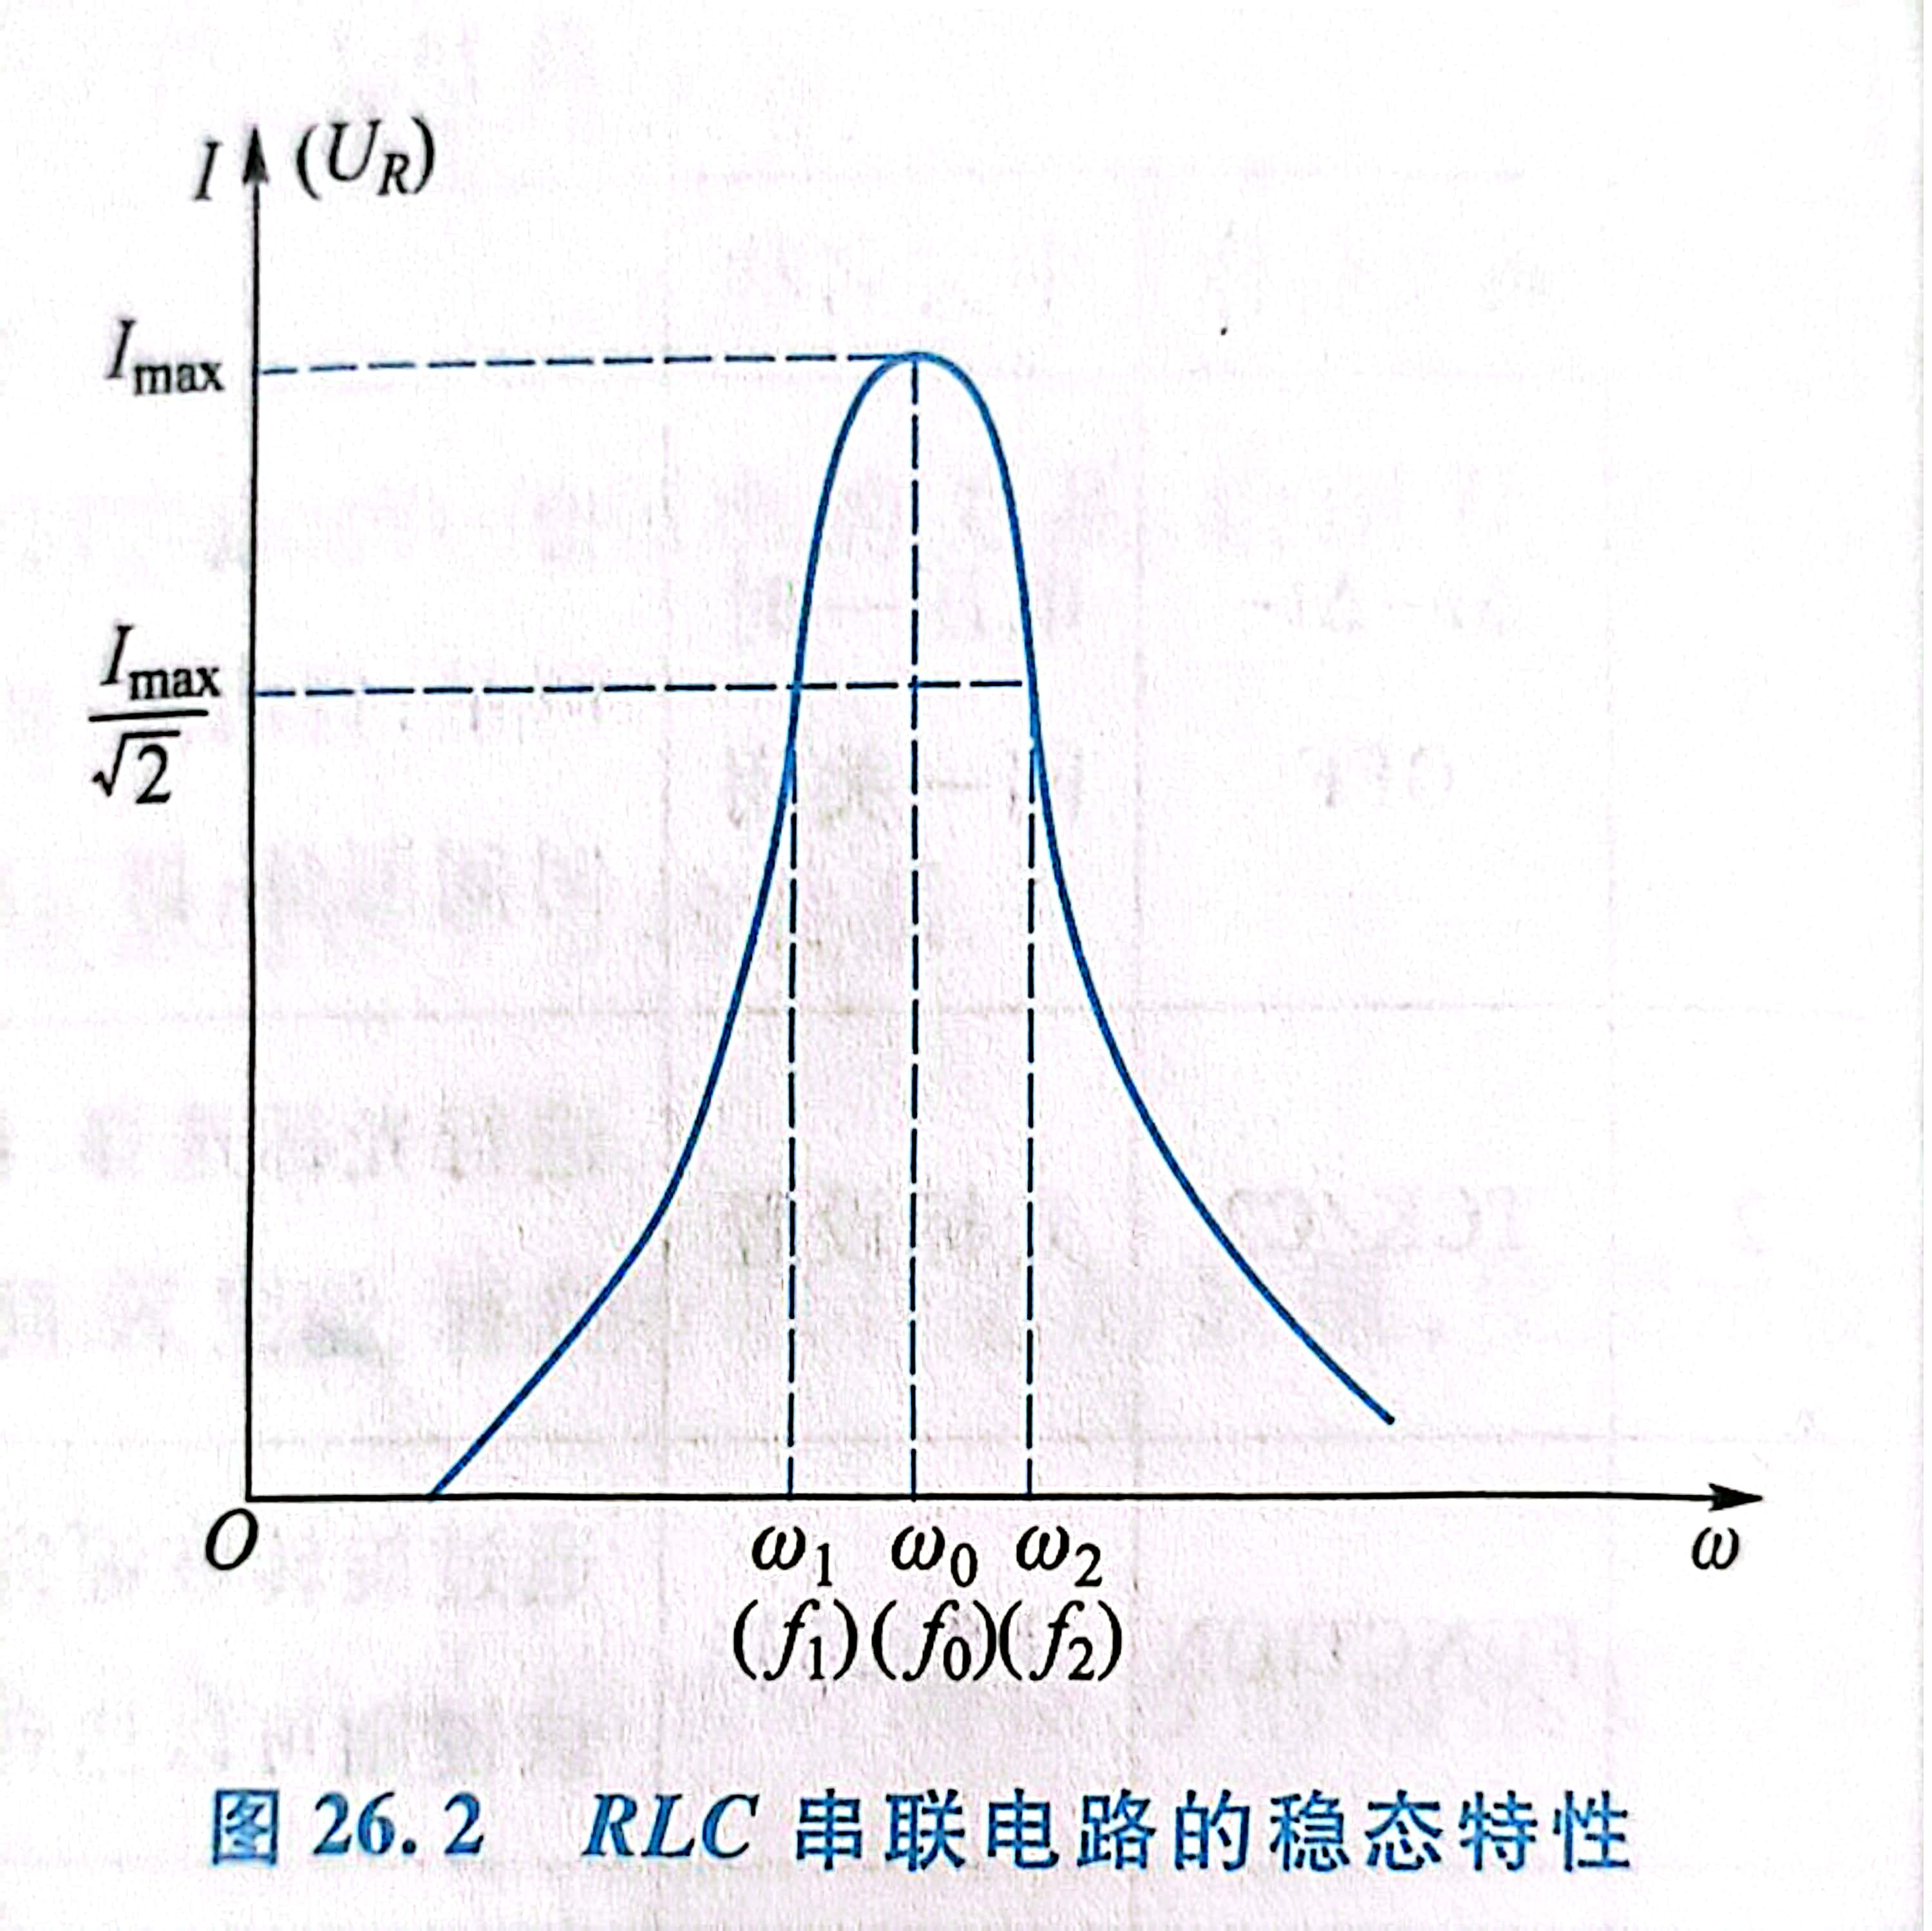
\includegraphics[width=\textwidth]{RLCwentaitexing.jpg}
  \end{minipage}
\end{figure}

\section{实验原理}
  \subsection{RLC传来内电路的幅频特性和相频特性}
  如图\ref{rlcdianlu},进行电路的连接。在电路中,电感线圈和电容器两者本身也具有损耗,
  和电阻在电路中的效果一样。
  所以现在设电感线圈和电容器两者串联后具有等效损耗电阻为$R_{L}$,则依照假设及电路,
  RLC电路中的总阻抗为
  \begin{equation}\label{rlczongzukang}
    Z=\sqrt{(R+R_{L})^2+(\omega L-\frac{1}{\omega C})^2}
  \end{equation}
  同时也能得出回路中的电流大小为
  \begin{equation}\label{rlcdianliu}
    I=\frac{U}{\sqrt{(R+R_{L})^2+(\omega L-\frac{1}{\omega C})^2}}
  \end{equation}

  保持总电压U不变,则会得到图\ref{rlcwentaitexing}所示的RLC串联电路的幅频特性曲线。
  由于欧姆定律$U=IR$,所以$U_{R}-\omega \mbox{和} I-\omega$关系是相同。因此实验
  中经常测量的是$U_{R}-\omega$曲线。

  实验中总电压和电流之间的相位差设为$\varphi$,可以表达为
  \begin{equation}\label{phibiaodashi}
    \varphi = \arctan \frac{\omega L-\frac{1}{\omega C}}{R+R_{L}} 
  \end{equation}
  
  \begin{wrapfigure}[13]{l}{4.5cm}\label{rlcxiangpintexing}
    \centering
    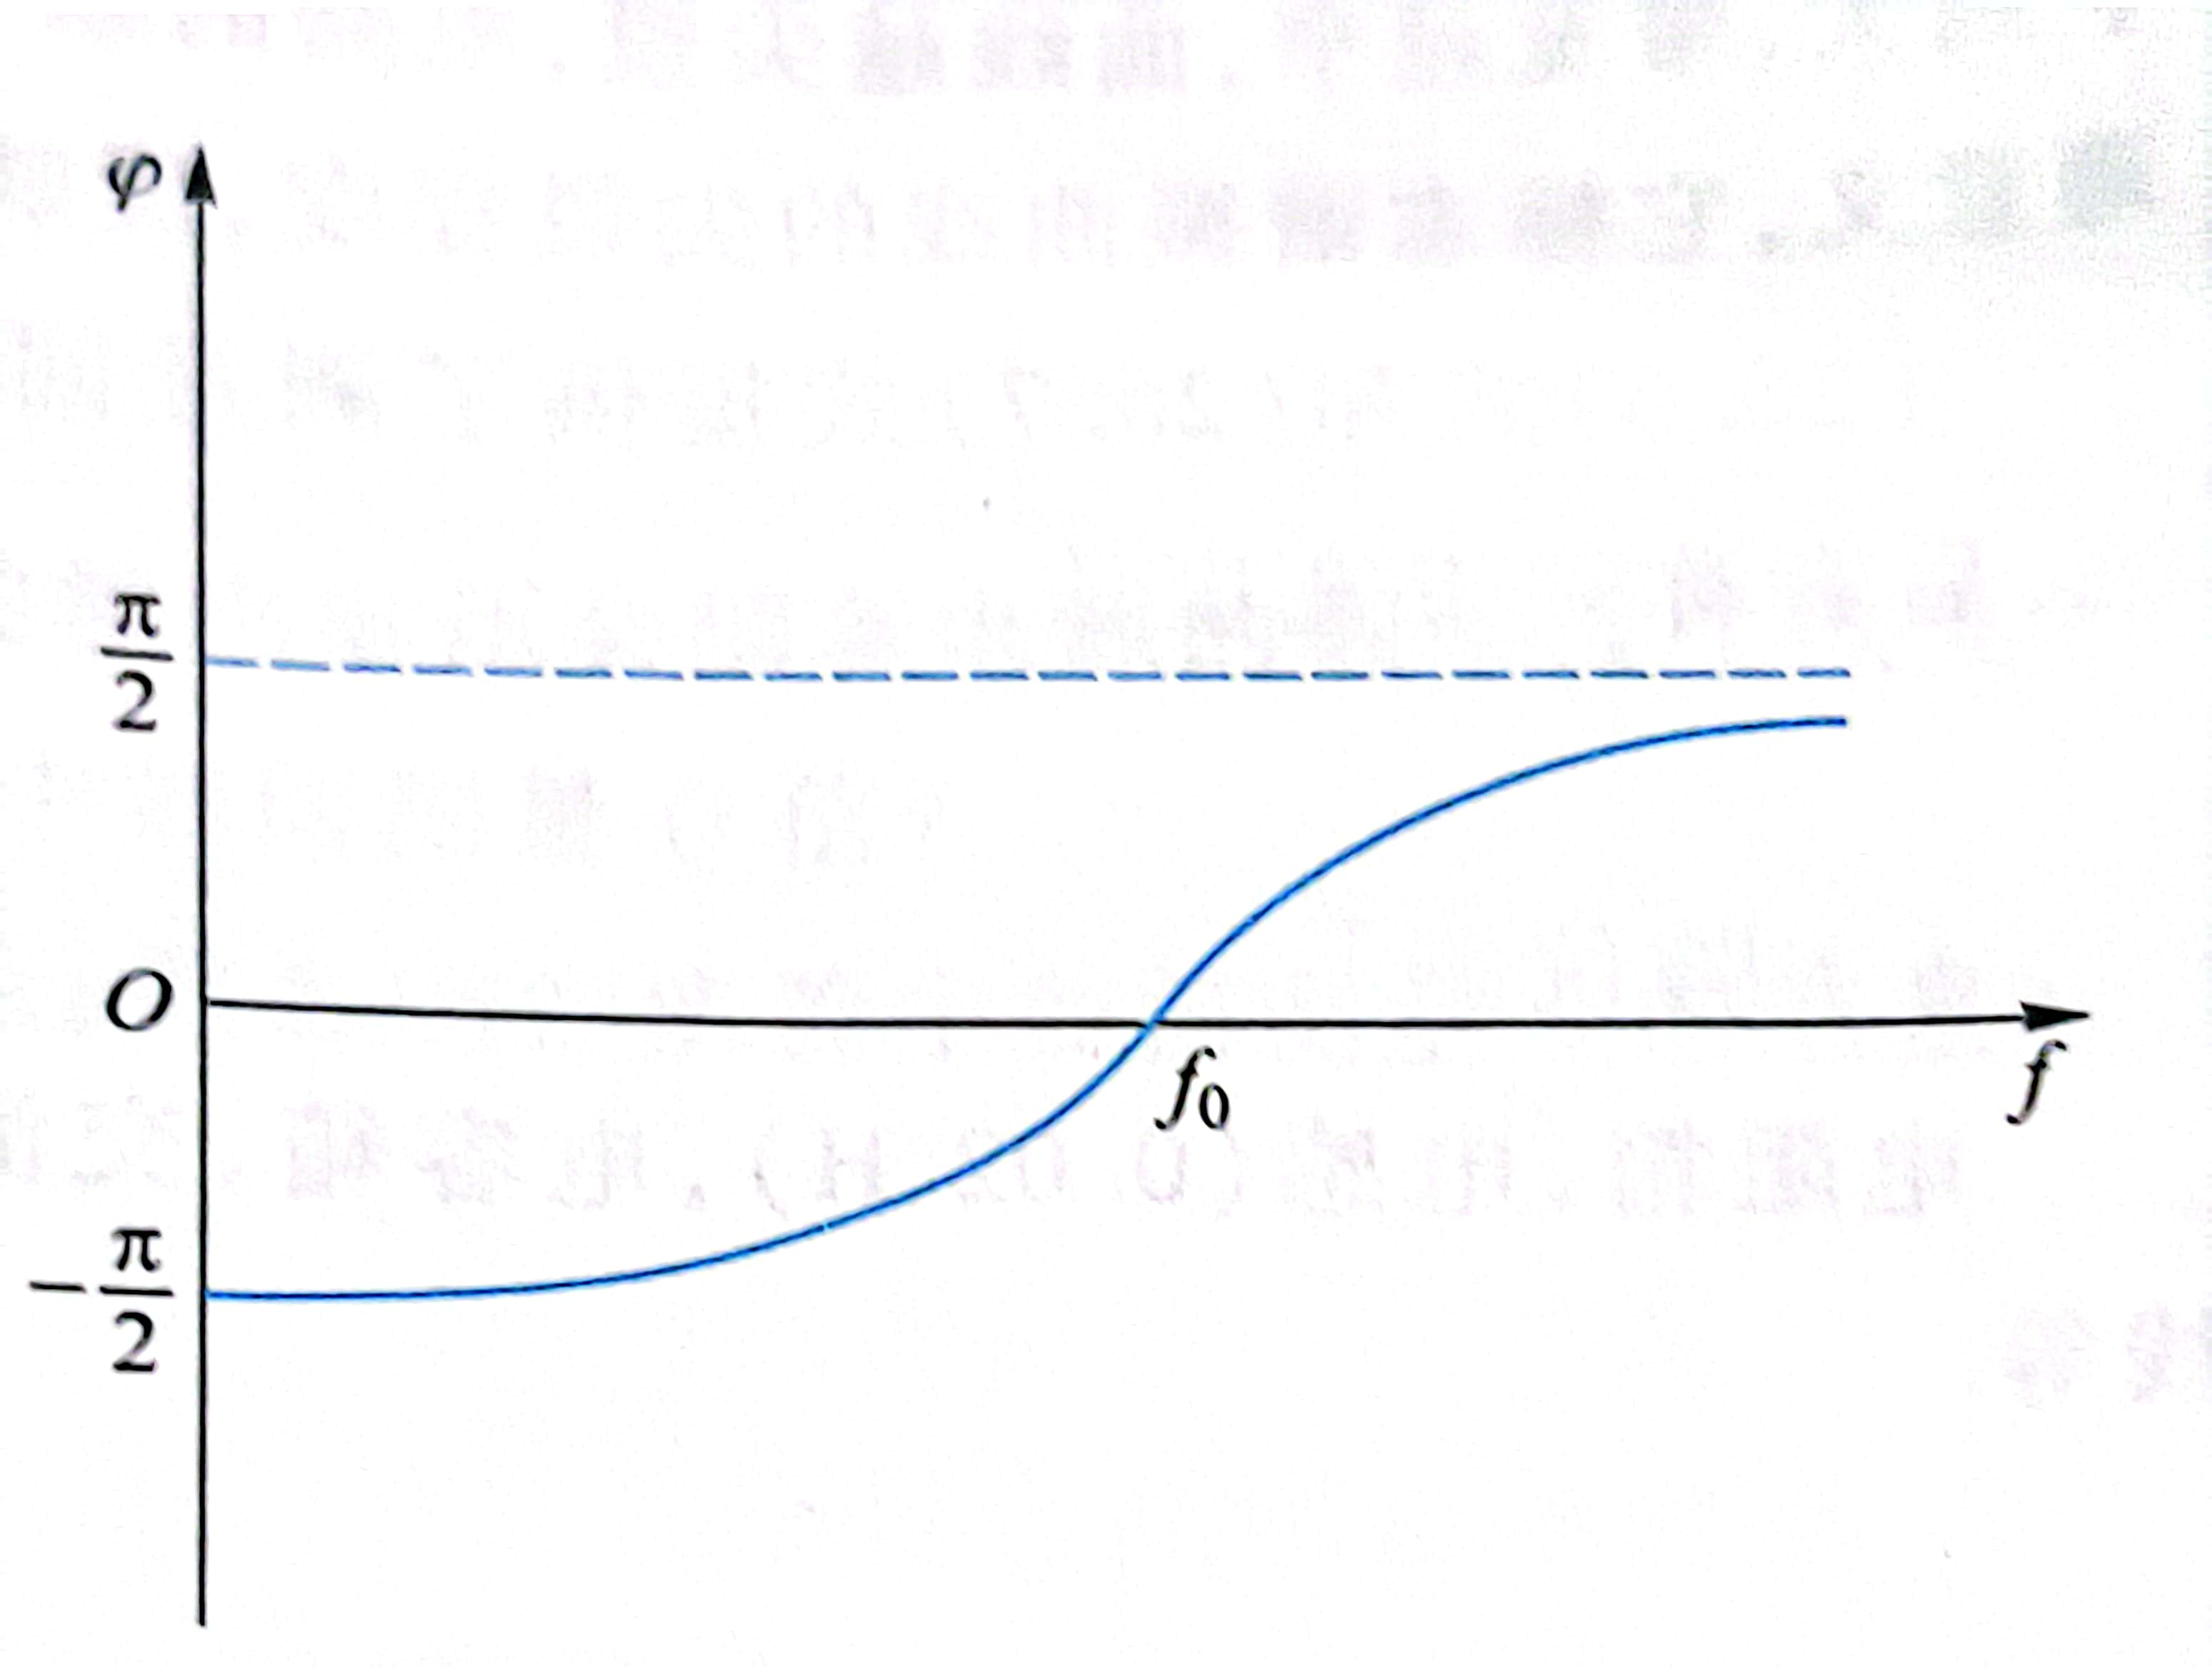
\includegraphics[width=0.3\textwidth,height=0.3\textheight]{RLCxiangpintexing.jpg}
    \caption{RLC相频特性}
  \end{wrapfigure}
  而实验中理论上应该出现的相位差随着电源频率变化关系如图\ref{rlcxiangpintexing}所展示的那样。
  从图\ref{rlcxiangpintexing}中以及$\varphi$的表达式式\ref{phibiaodashi}可以得出以下结论:

  1.\quad  当$\omega L > \frac{1}{\omega C}$时,有$\varphi > 0$,电流的相位落后于电源电压,整个电路
            呈现电感性,随着频率的增加$\varphi$越来越接近$\frac{\pi}{2}$。
            电感性的意思就是:
            电感性是指导体中的电流变化时会引起该导体中的自感应电动势的性质。
            从物理意义上看,电感性是描述导体中电磁场的建立和消散过程。当电流在导体中变化时,
            围绕导体的磁场也随之变化,而磁场的变化又会在导体内部感应出电动势,这个过程就体现了电感性。

  2.\quad  当$\omega L < \frac{1}{\omega C}$时,有$\varphi < 0$,电流的相位超前于电源电压,整个电路
            呈现电容性,随着频率的减小,$\varphi$越来越接近$\frac{\pi}{2}$。
            电容性是指导体对电荷的储存能力的一种性质。
            从物理意义上讲,电容性反映了导体中的电荷和电势之间的关系。当在导体上的两点之间存在电势差时,
            会在导体的两点附近聚集对应量的正负电荷,这种聚集电荷的能力就是电容性。

  3.\quad  当$\omega L = \frac{1}{\omega C}$时,有$\varphi < 0$,电流相位等于电源电压。整个电路
            处于谐振状态,此时回路中电流达到最大,记作$I_{max}$,令$\omega_{0}\mbox{和}f_{0}$分别表示
            $\varphi = 0$时候的角频率和频率,并分别成为谐振角频率和谐振频率,也可以表达为
            \begin{equation}
              \omega_{0}=\frac{1}{\sqrt{LC}} \mbox{,} f_{0}=\frac{1}{2\pi \sqrt{LC}}
            \end{equation}
  
  \subsection{RLC串联谐振电路的品质因素Q}
  当RLC串联谐振的时候,也就是出现当$\omega L = \frac{1}{\omega C}$时,
  有$\varphi < 0$,电流相位等于电源电压的时候,$U_{L}=U_{C}$,即纯电感和理想电容两端的电压相等,而
  \begin{equation}
    U_{L}=I_{max}\omega_{0}L=\frac{U}{R+R_{L}}\omega_{0} L=\frac{U}{R+R_{L}}\sqrt{\frac{L}{C}}
  \end{equation}
  令$Q=\frac{1}{R+R_{L}} \sqrt{\frac{L}{C}}$则有
  \begin{equation}\label{qyiyi}
    U_{L}=U_{C}=QU
  \end{equation}
  Q称为串联谐振电路的品质因数,式中的U为信号源的输出电压,如果Q>>1,则$U_{L}$和$U_{C}$都远大于信号源电压。
  这种现象叫做RLC电路的电压谐振。Q值反映了谐振电路的特性,由式\ref{qyiyi}得到Q的一个物理意义:
  电压谐振时,电路呈纯电阻性,纯电感和理想电容两端的电压均为信号源电压的Q倍。

  为了描述$I-\omega$谐振曲线的尖锐程度,通常规定I由最大值$I_{max}$下降到$\frac{I_{max}}{\sqrt{2}}$时
  对应的频率$\omega_{1}$和$\omega_{2}(\omega_{1}<\omega_{0}<\omega_{2})$之差称为“通频带宽都”,与$\omega_{0}$
  和回路的品质因数Q之间的关系为
  \begin{equation}\label{qyiyi2}
    Q=\frac{\omega_{0}}{\omega_{2} - \omega_{1}}=\frac{f_{0}}{f_{2}-f_{1}}
  \end{equation}
  Q越大,带宽越窄,曲线越尖锐,电路的频率选择性越好,由此得到的Q值的第二个物理意义:它标志谐振曲线的尖锐
  程度,反映电路对频率的选择性。

  式\ref{qyiyi}和式\ref{qyiyi2}提供了测量回路Q值的原理和方法,前者称为电压谐振法,后者称为频带宽度法。

\section{实验装置器材介绍}
电阻箱、电感(0.02H)、电容箱、交流信号源、交流毫伏表、双通道示波器、导线等

\section{实验内容及实验步骤}
  \subsection{测量RLC串联电路的幅频特性和相频特性}
  \ding{172} 按照图\ref{rlcdianlu}连接电路,选择合适LC的数值。

  \ding{173} 使用示波器的两个通道同时观察电源和电阻两端的电压,根据公式先估算以下电路的谐振频率$F_{0}$,
              然后调节信号源的频率,观察电阻两端电压岁频率的变化规律,确定测量频率范围。

  \ding{174} 以一定的频率间隔从低到高改变频率,每一个频率测量点测量电阻两端的电压$U_{R}$和电阻两端
              电压与电源电压之间的相位差$\varphi_{R}$,在测量过程中注意保持电源电压幅值的稳定。

  \ding{175} 绘制RLC串联电路的谐振曲线$U_{R}-f\mbox{和}\varphi_{R}-f$

  \subsection{测量回路的品质因数Q值}
  \ding{172} 当电路处于谐振状态时,将电容与电阻交换位置,测量电容两端的电压$U_{C}$。或将电感和电阻交换位置,
              测量电感两端的电压$U_{L}$,计算品质因数Q。

  \ding{173} 在$U_{R}-f$图上画出RLC串联电路的频带宽度,并计算Q值。

  \ding{174} 将Q的测量值和计算值进行比较。
\newpage

\section{实验原始数据}
\begin{figure}[H]
  \centering
  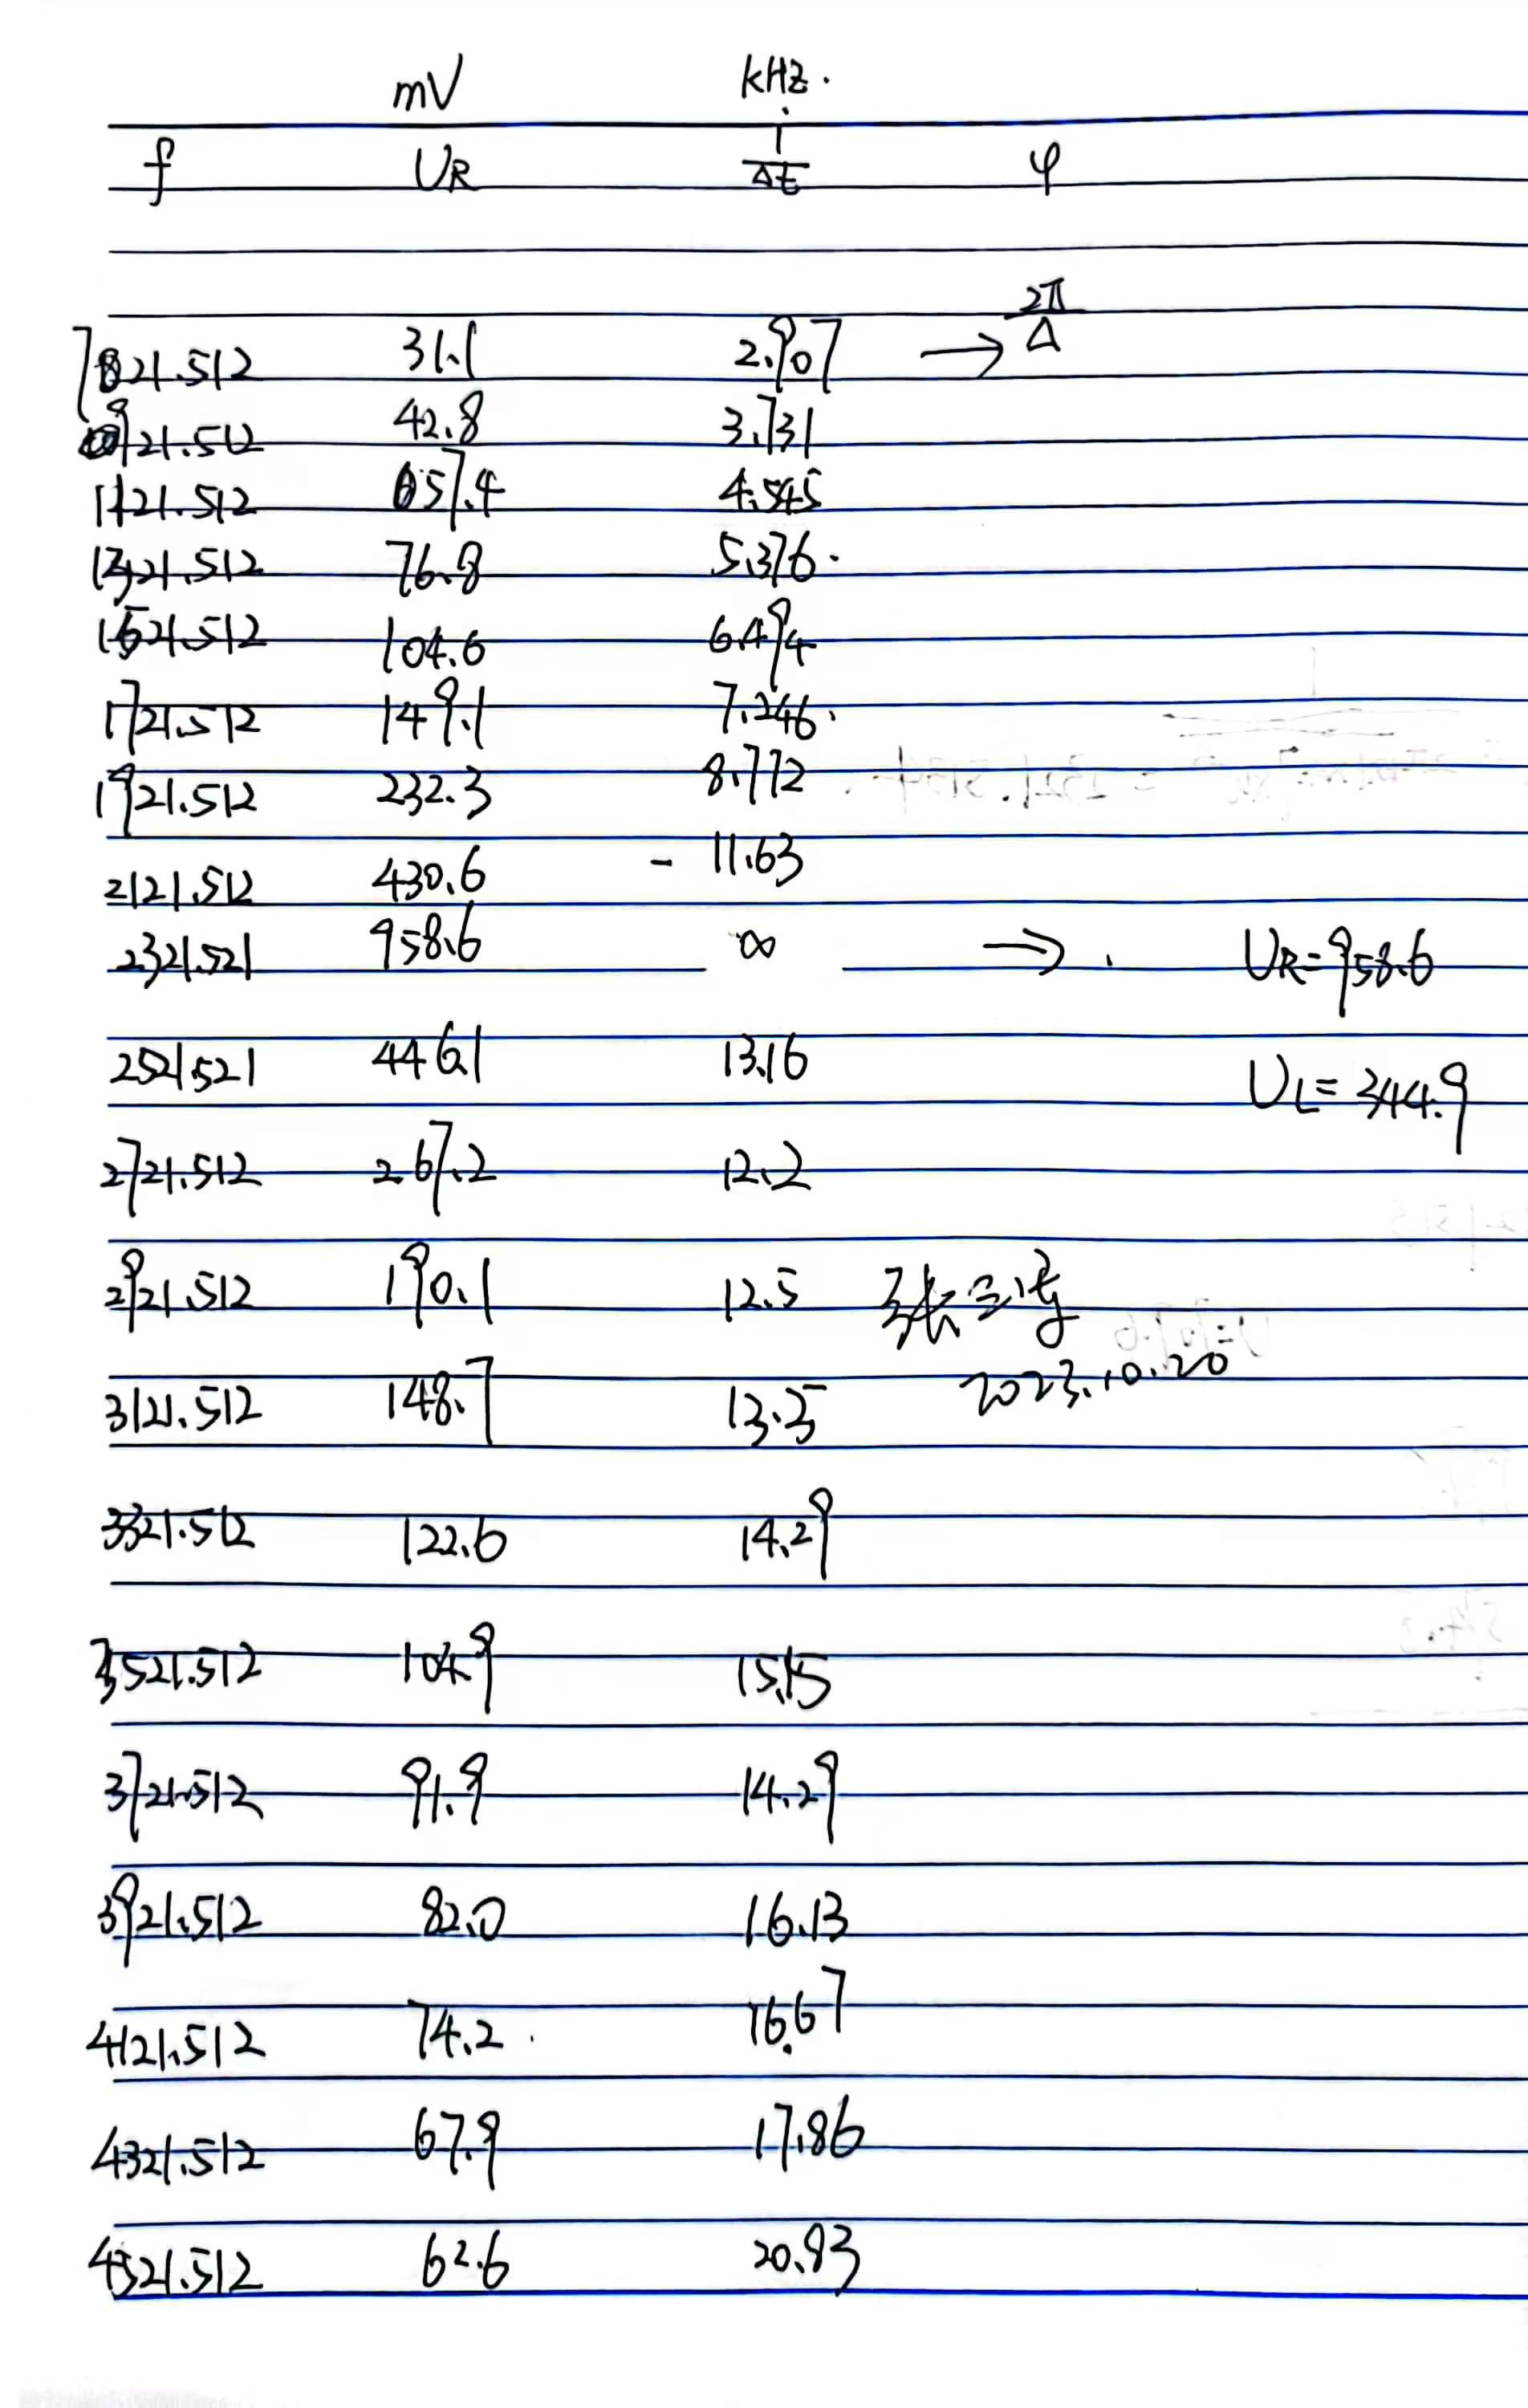
\includegraphics[width=0.9\textwidth,height=0.8\textheight]{yuanshishujv.jpg}
  \caption{实验原始数据1}
\end{figure}
\newpage


\section{实验数据处理}
  \subsection{测量RLC串联电路的幅频特性和相频特性}
  实验中使用的器材如图\ref{qicai}
  \begin{figure}[htbp]\label{qicai}
    \begin{minipage}[t]{0.45\textwidth}
    \centering
    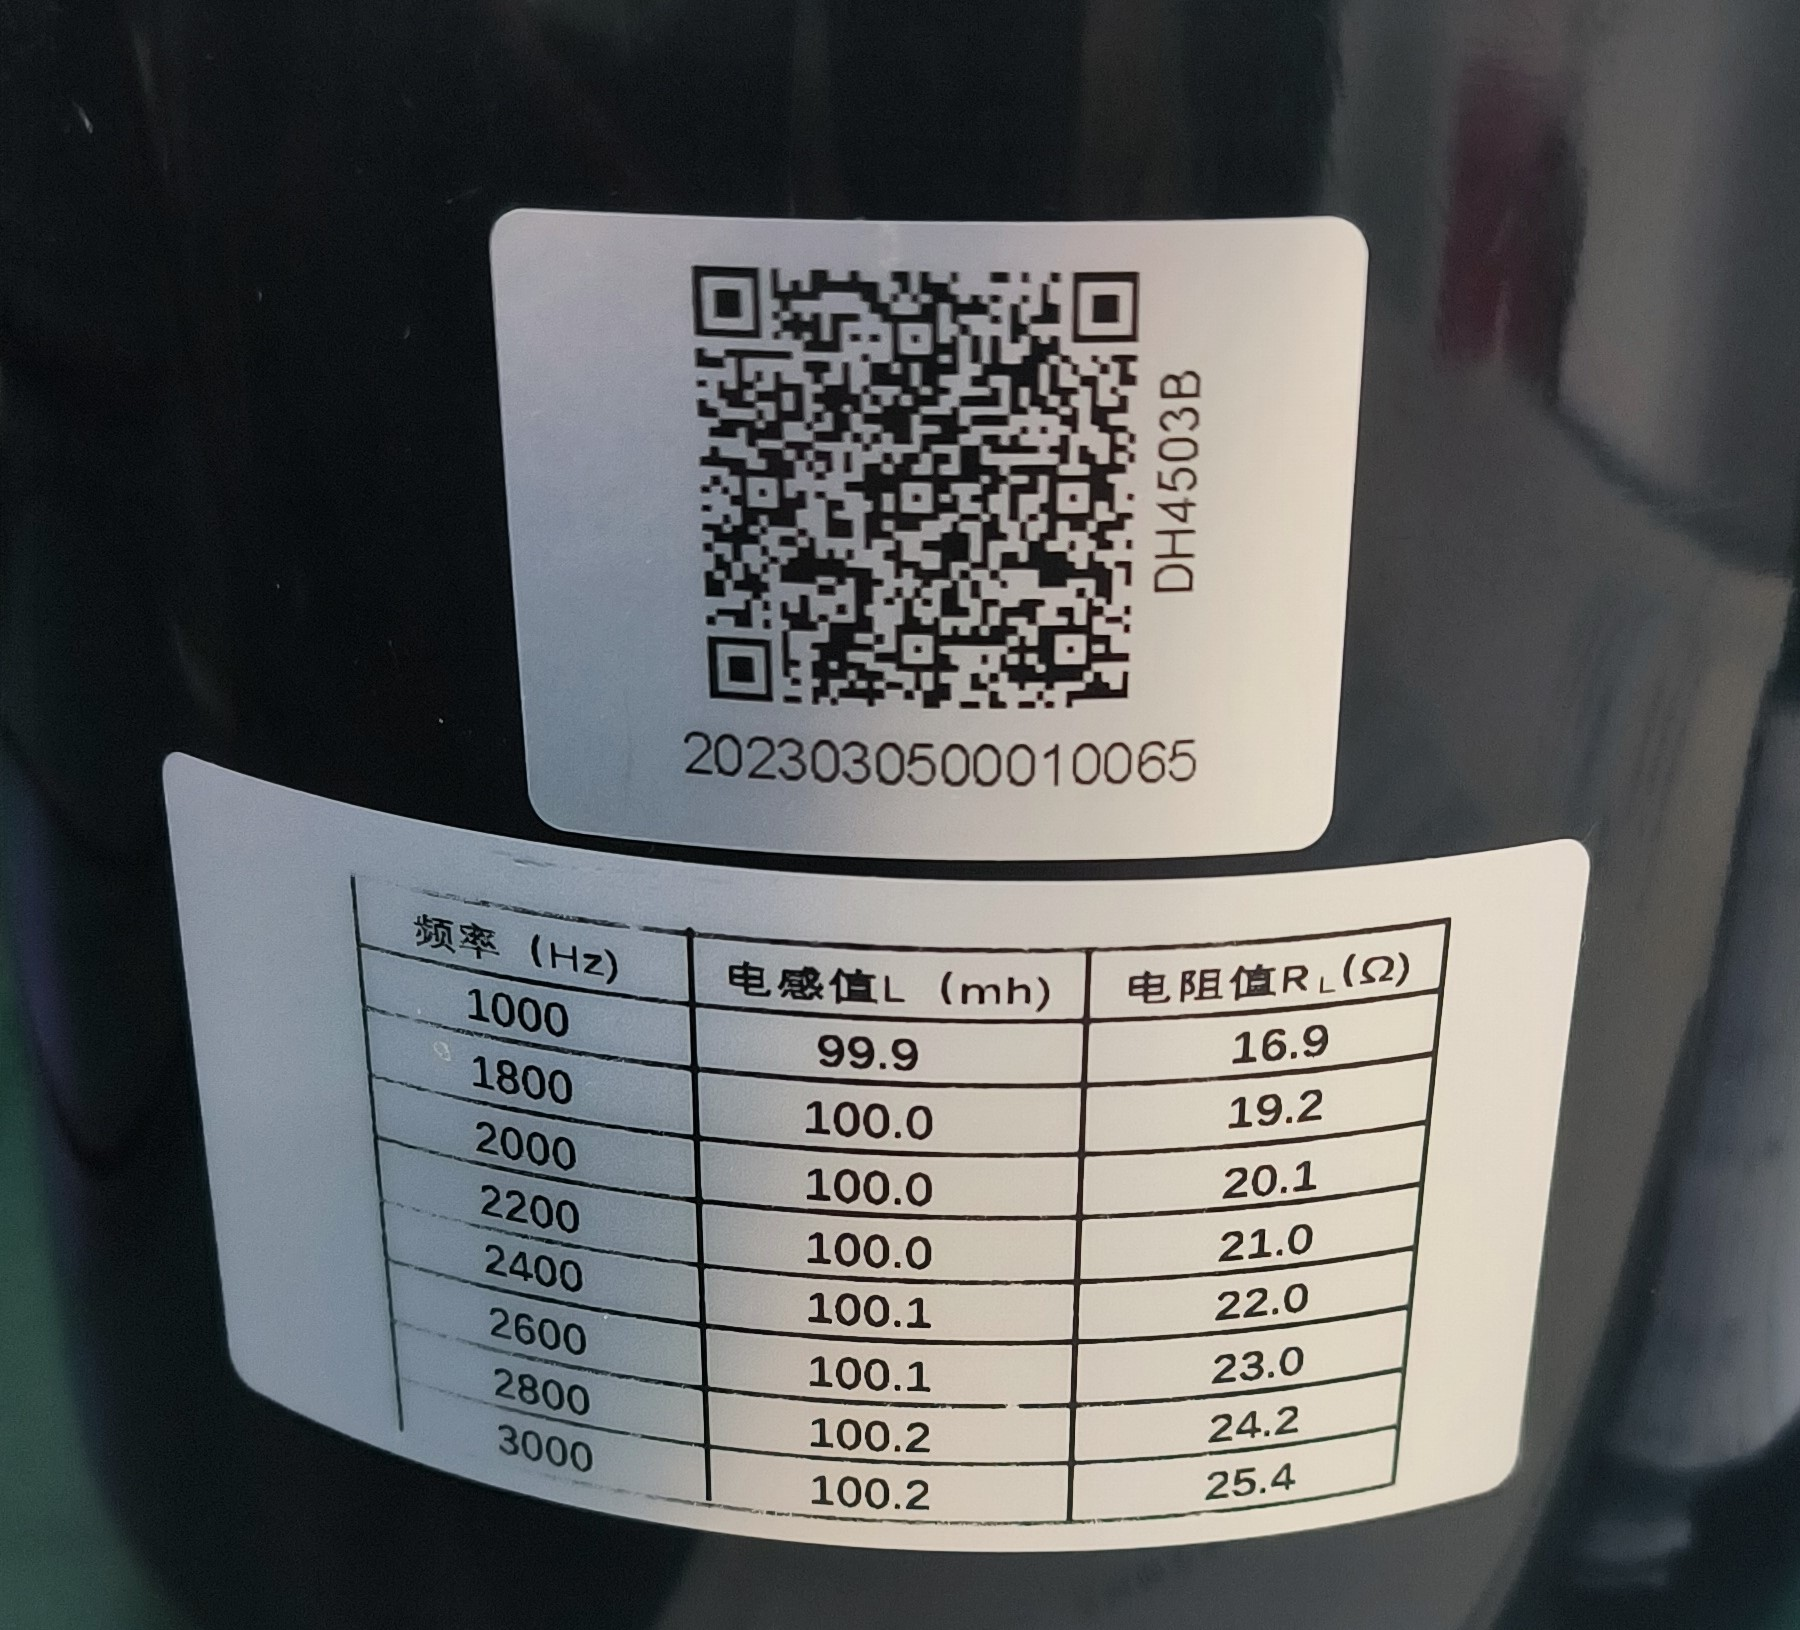
\includegraphics[width=\textwidth]{qicai1}
    \end{minipage}
    \hfill
    \begin{minipage}[t]{0.45\textwidth}
    \centering
    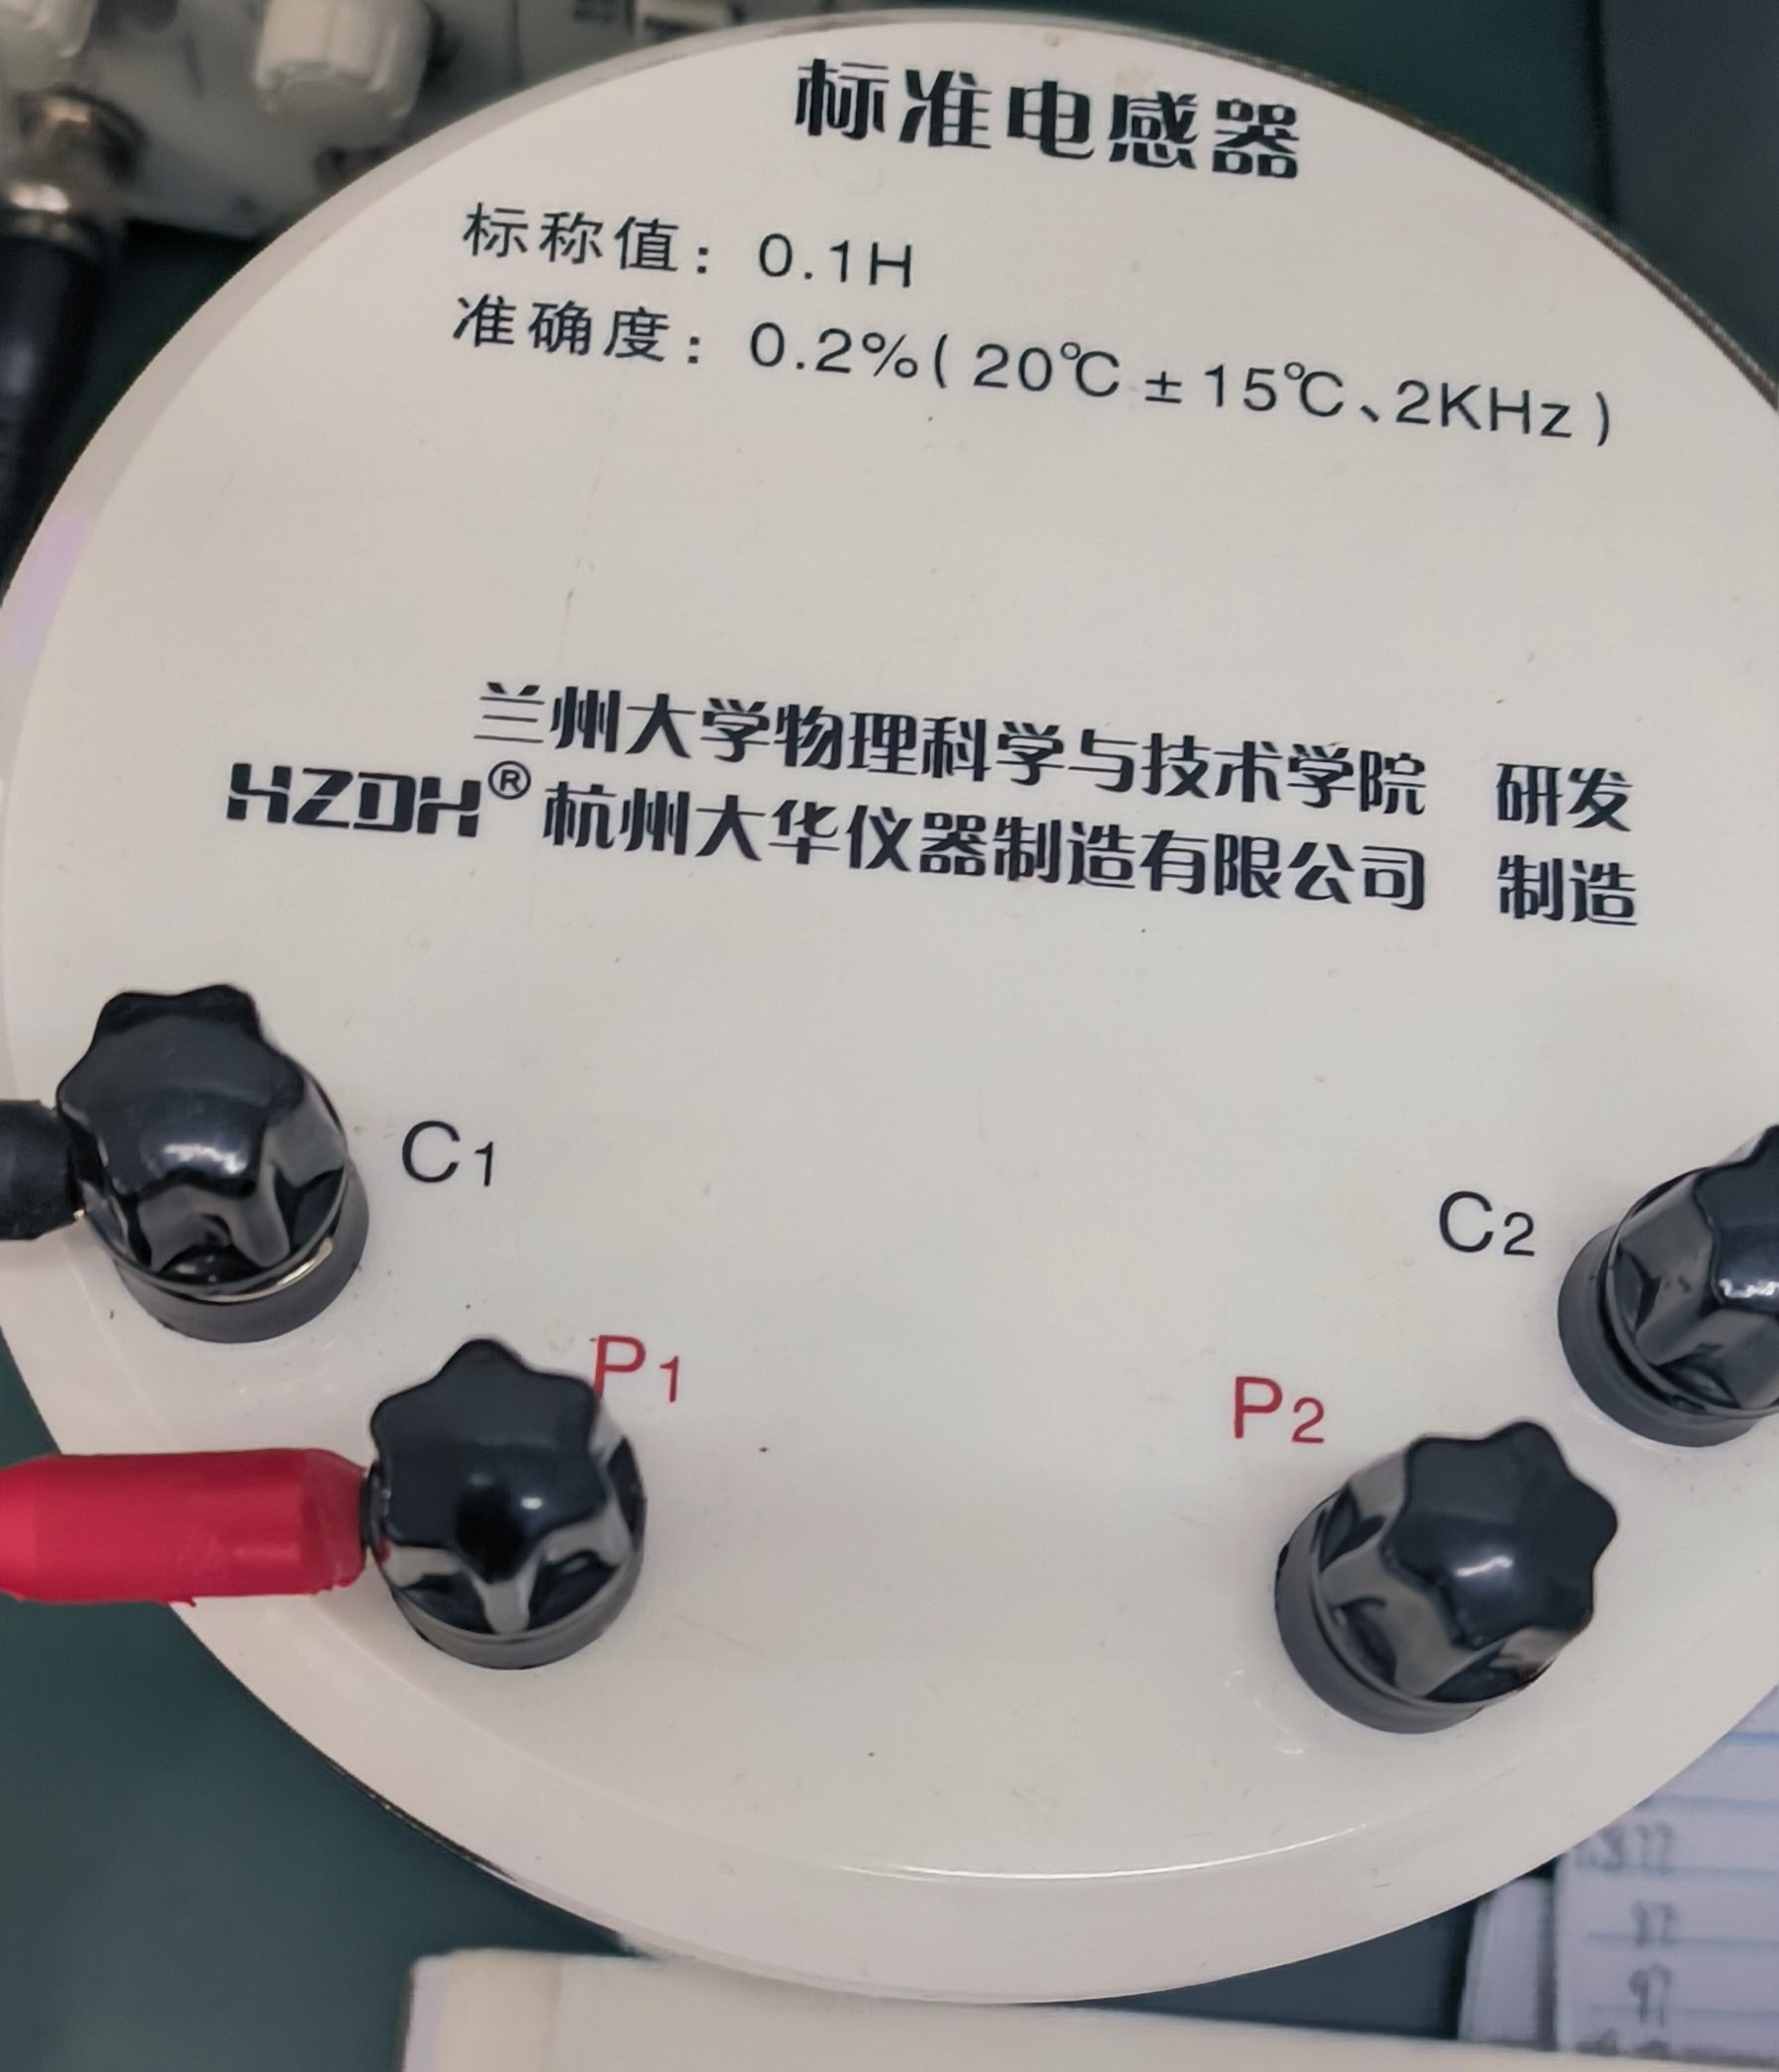
\includegraphics[width=\textwidth]{qicai2}
    \end{minipage}
    
    \begin{minipage}[t]{0.45\textwidth}
    \centering
    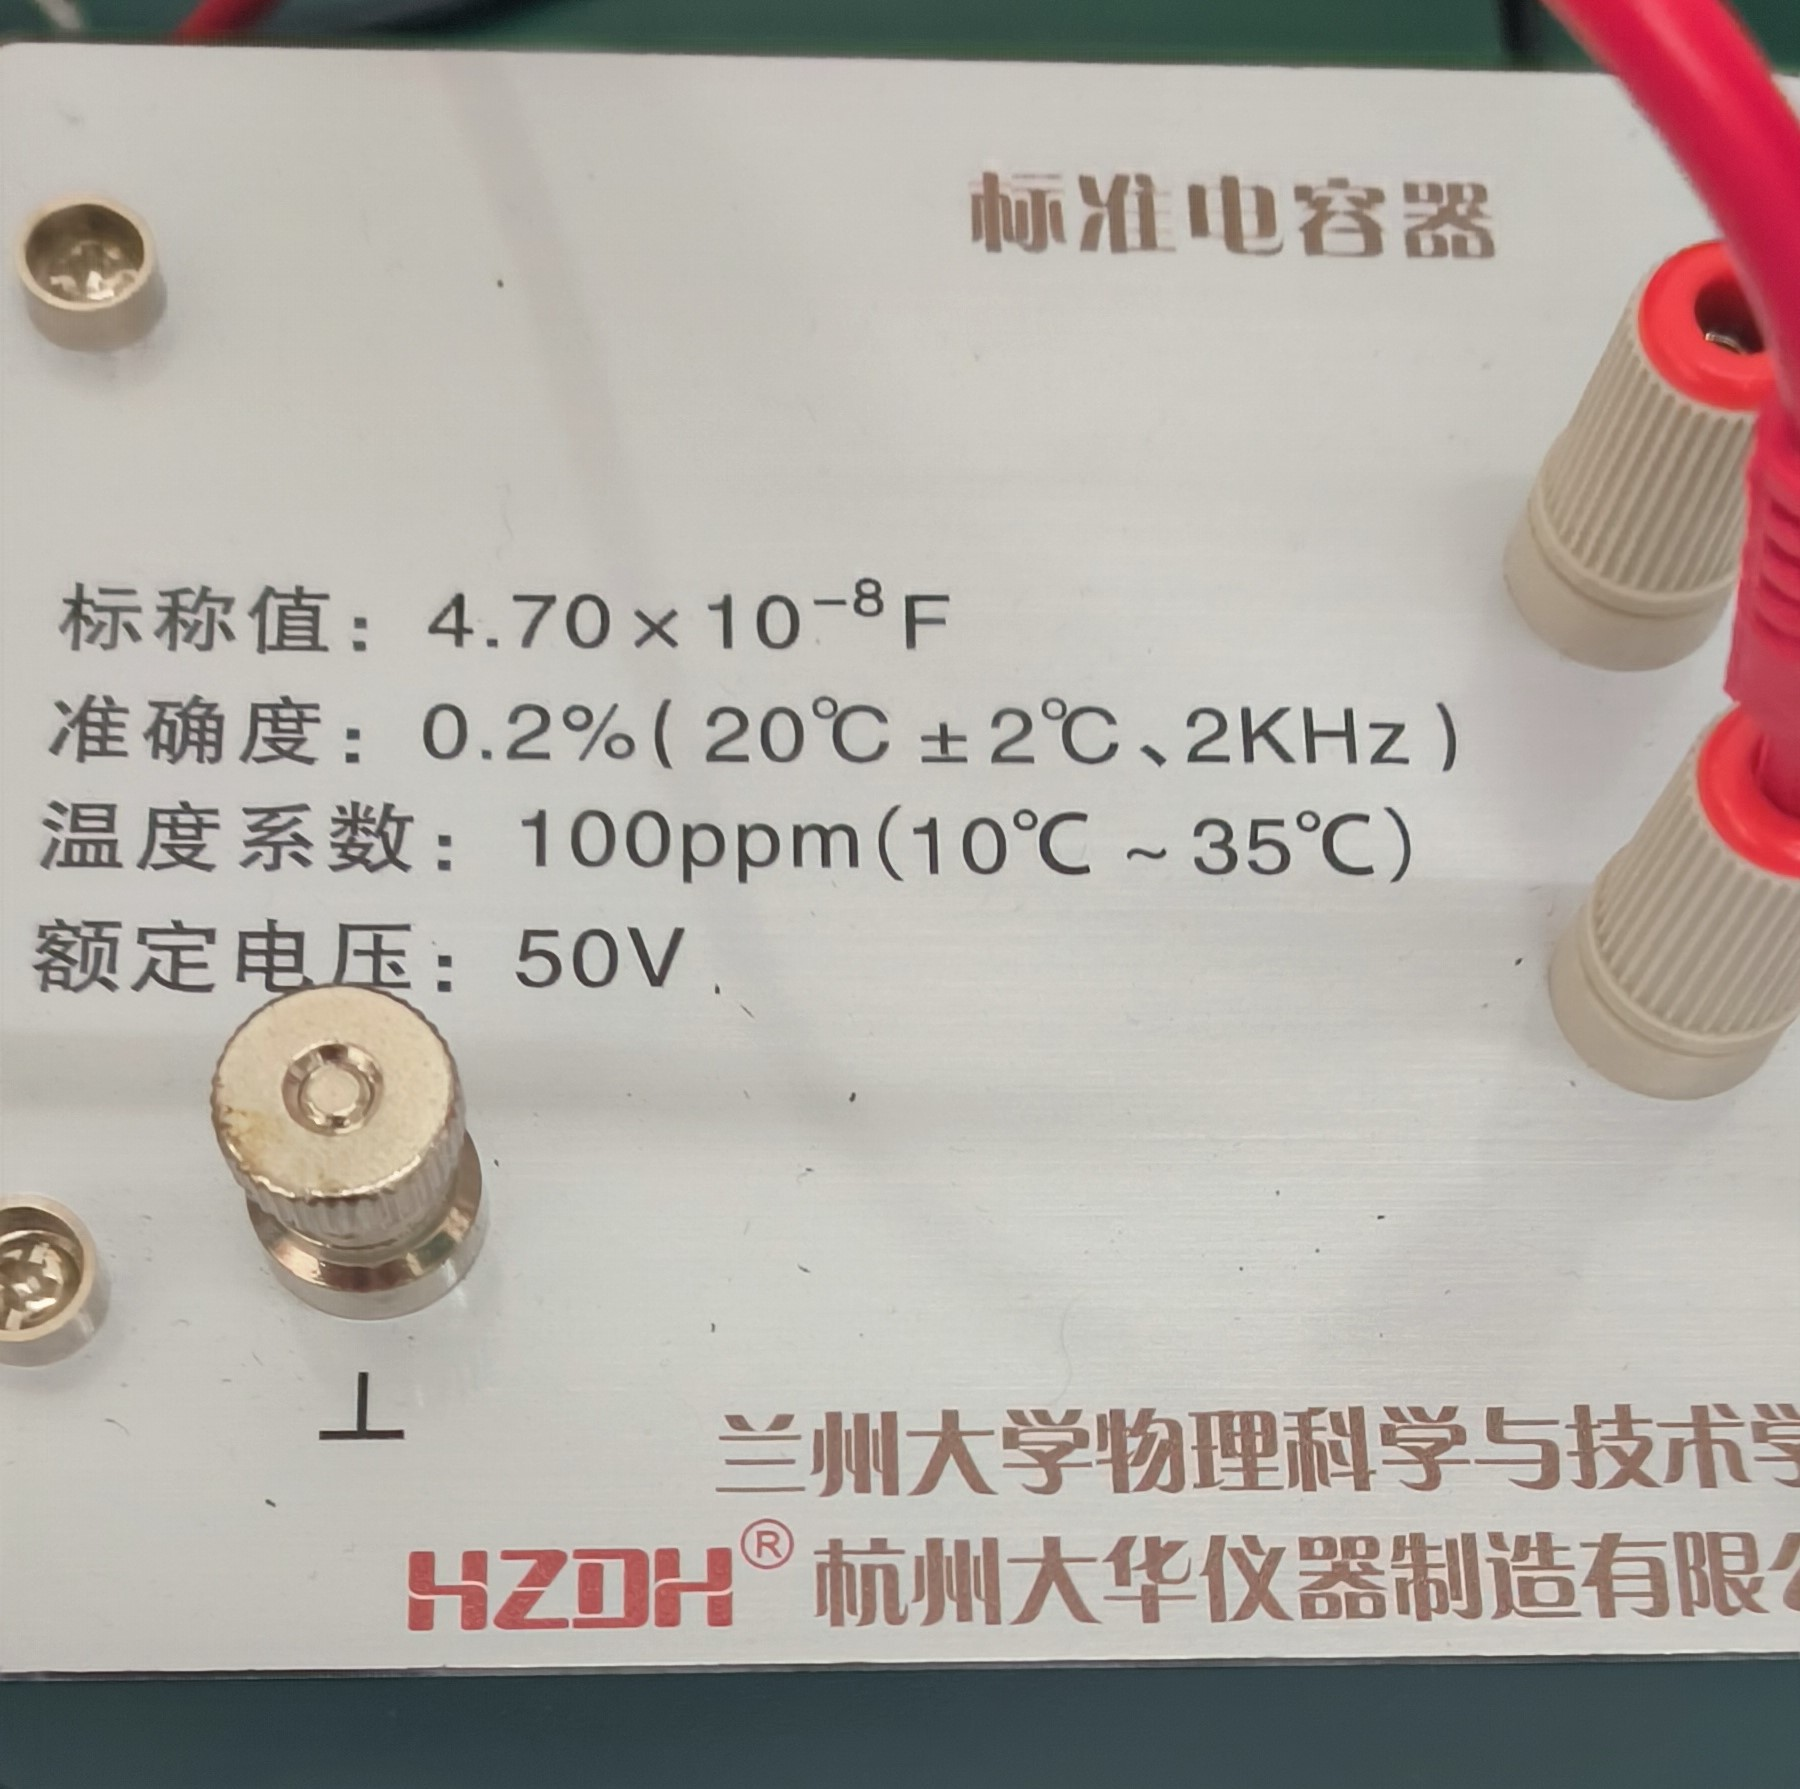
\includegraphics[width=\textwidth]{qicai3}
    \end{minipage}
    \hfill
    \begin{minipage}[t]{0.45\textwidth}
    \centering
    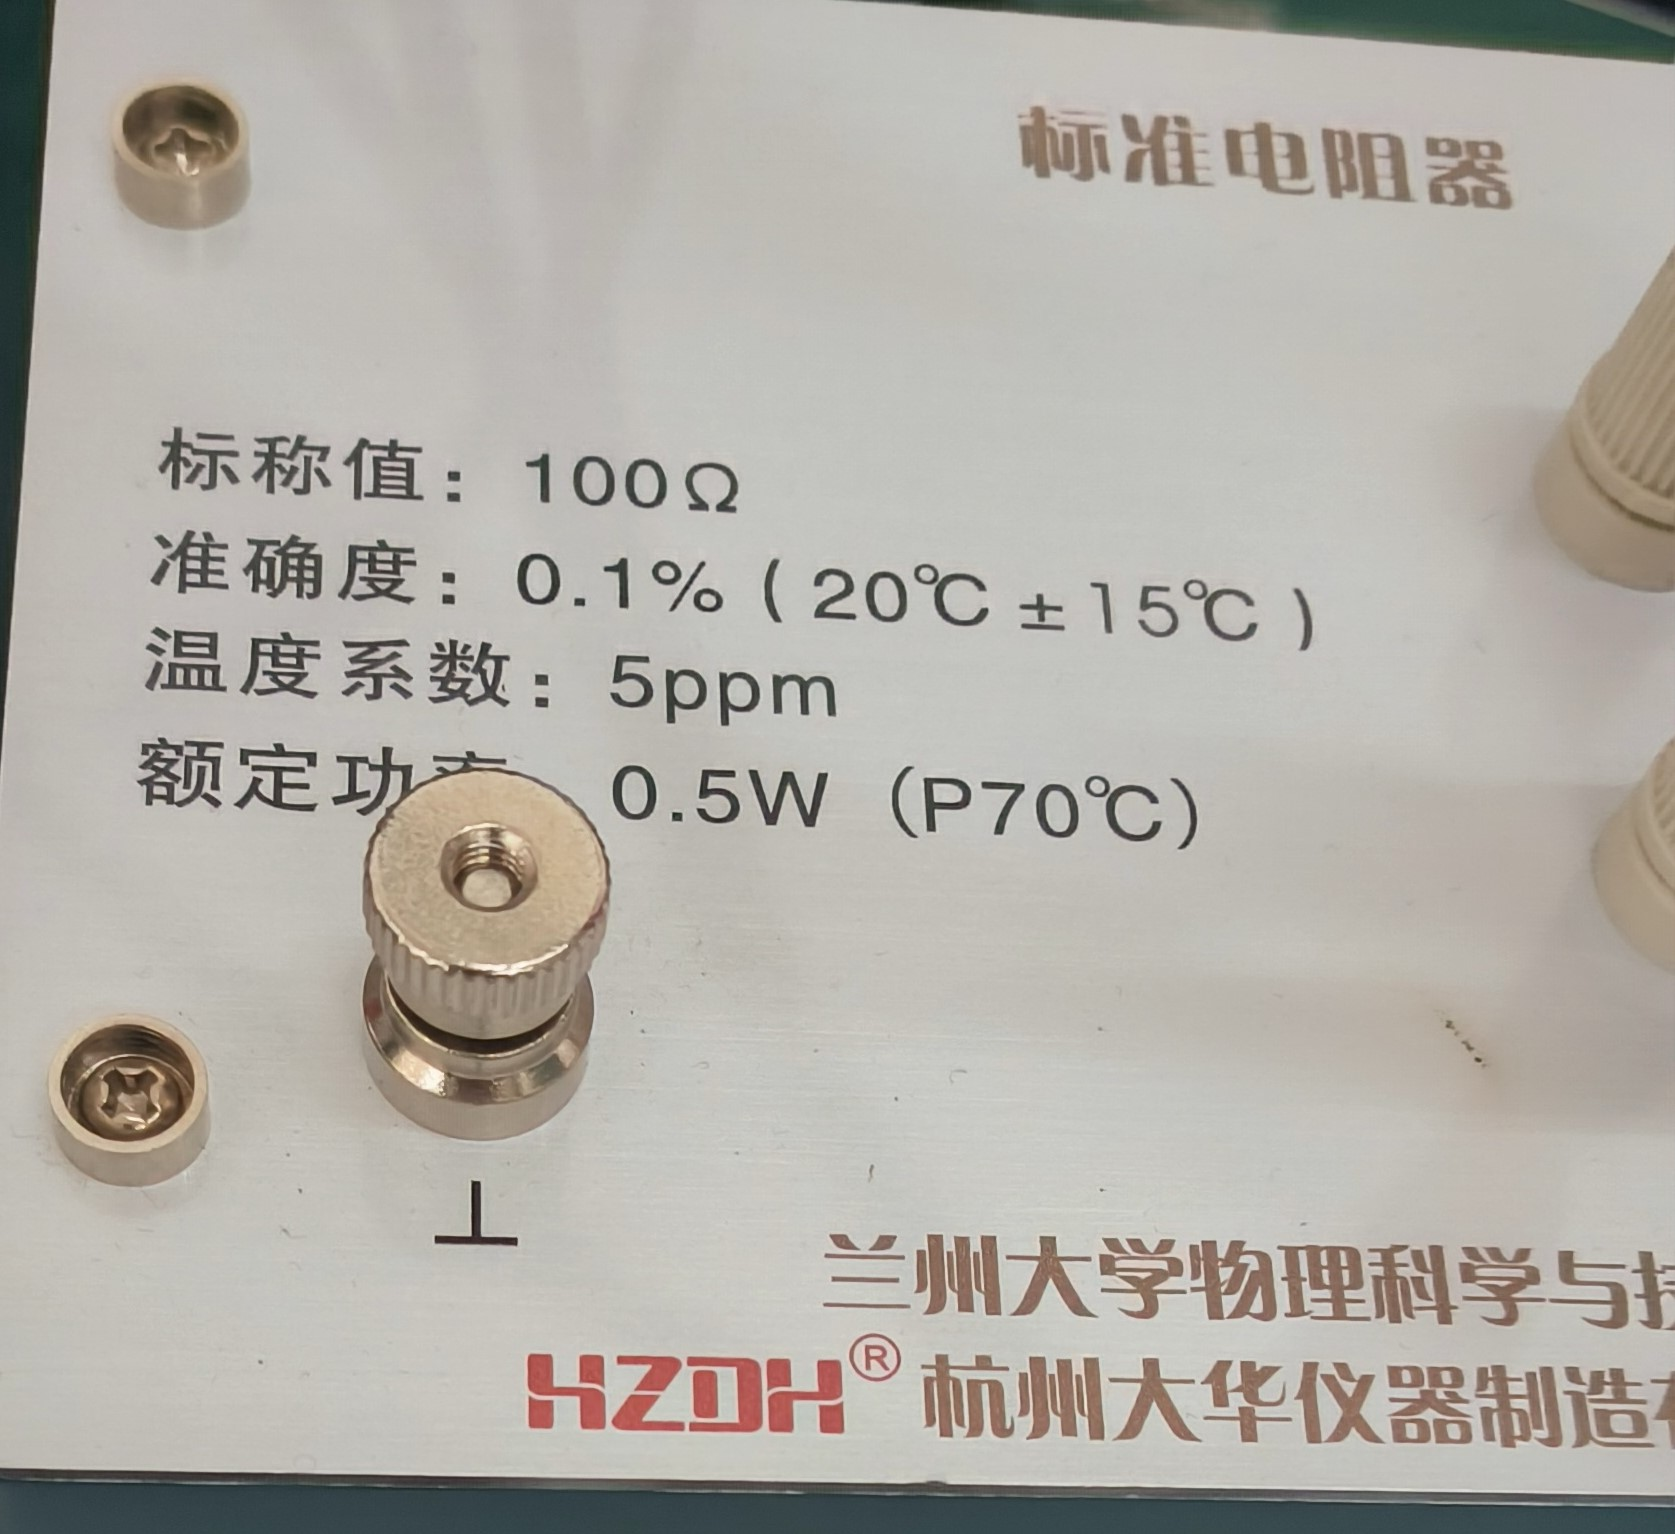
\includegraphics[width=\textwidth]{qicai4}
    \end{minipage}
    \caption{实验所用器材展示}
    \end{figure}

  \begin{figure}[H]\label{shujv}
    \centering
    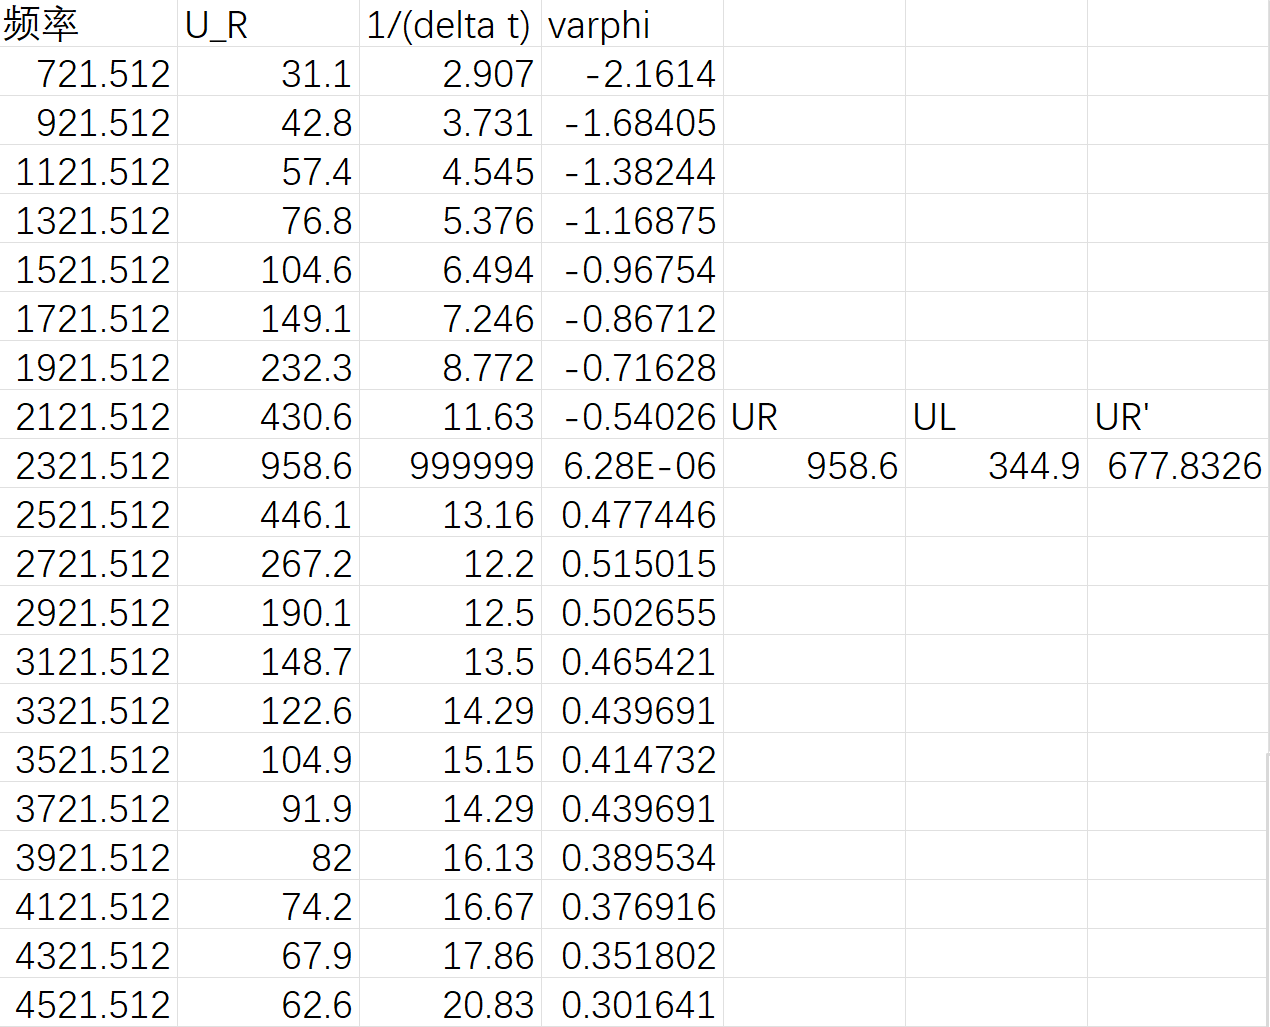
\includegraphics[width=0.6\textwidth,height=0.4\textheight]{shujv.png}
    \caption{实验数据}
  \end{figure}

  \begin{figure}[H]\label{zuotu}
    \centering
    \begin{minipage}{\linewidth}
    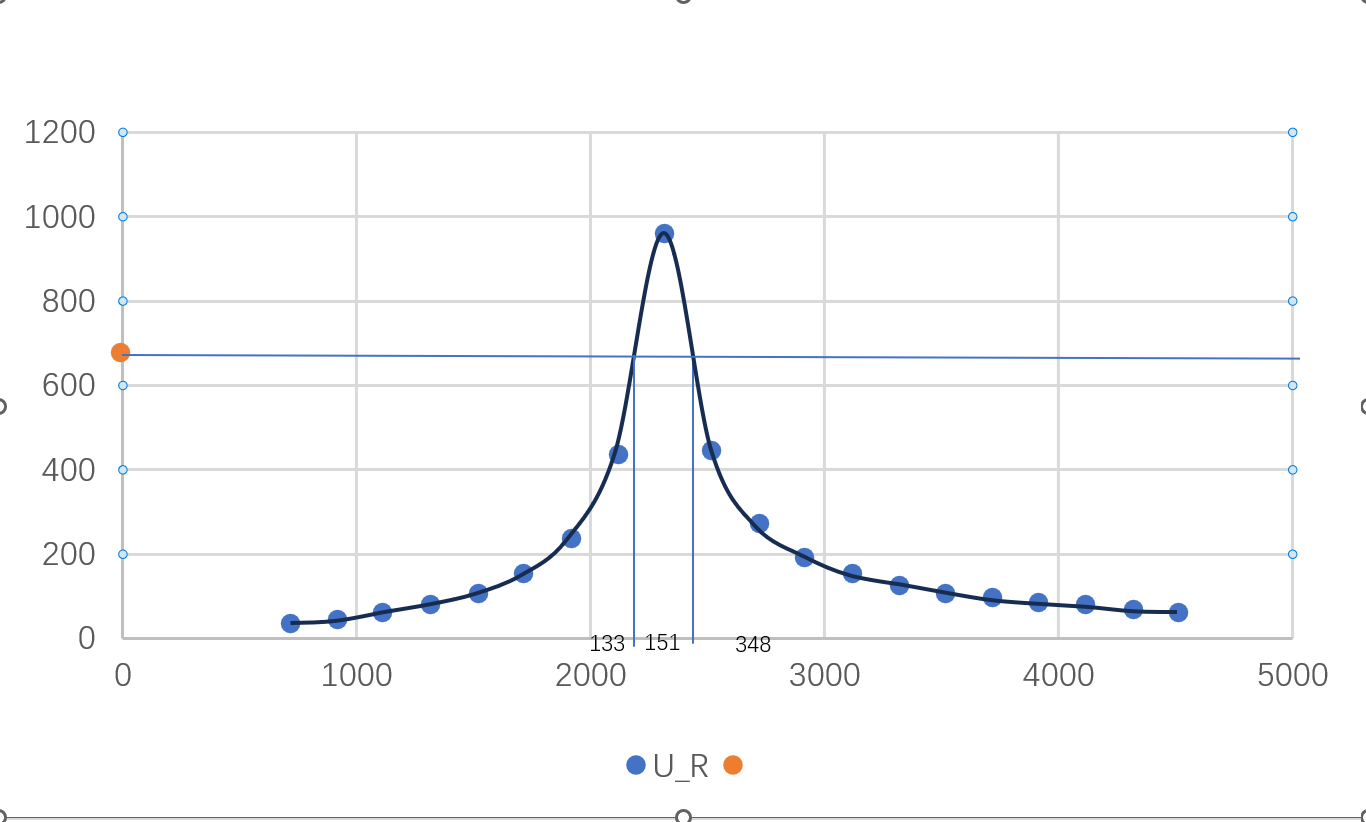
\includegraphics[width=0.47\textwidth,height=0.3\textheight]{f_ur_zuotu.png}\hfill
    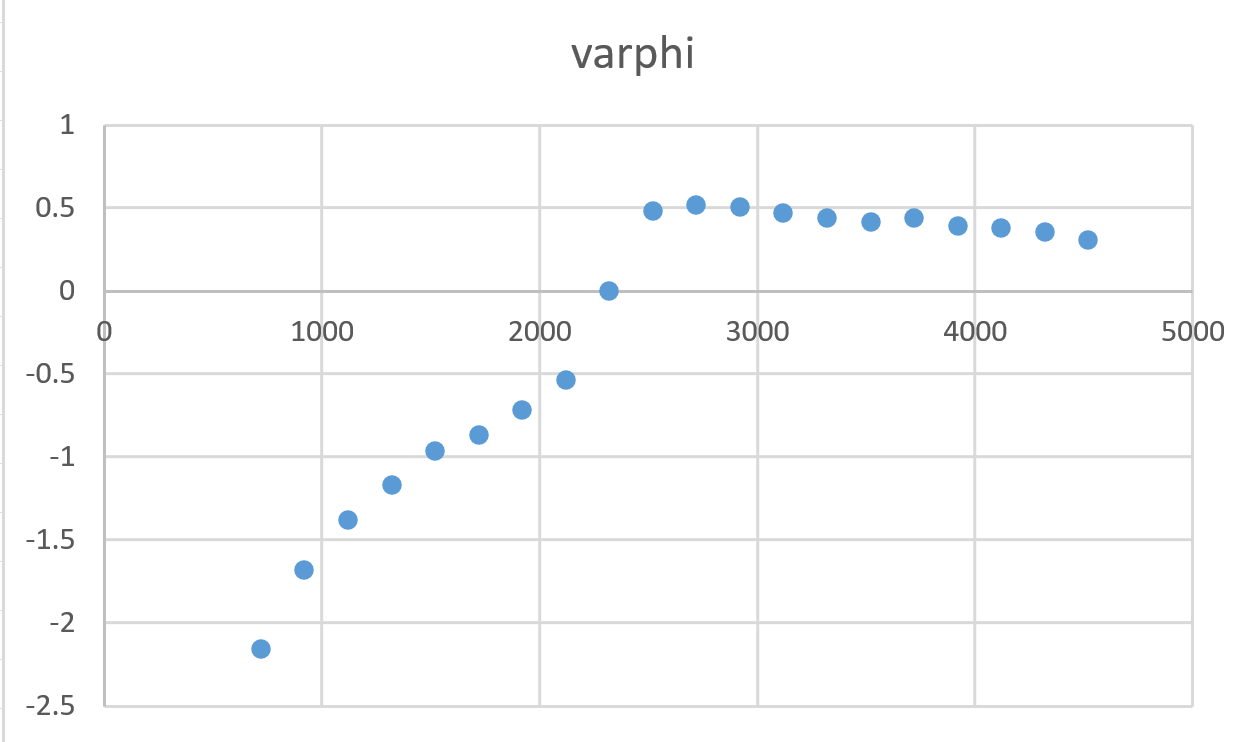
\includegraphics[width=0.47\textwidth,height=0.3\textheight]{f_varphi_zuotu.png}\hfill
    \end{minipage}
    \caption{$U_{R}-f$图形及$\varphi - f$图形}
  \end{figure}

  实验结果如图\ref{shujv}所示,进行图像处理,在坐标轴上画出数据点获得图\ref{zuotu}。

  最终实验结果中$U_{R}-f$图形较为符合预期,实验较为成功。而$\varphi - f$图形结果较为失败,图形形状
  不符合预期图像。

  最终得到的结果误差较大,出现明显图像偏移扭曲,分析误差产生原因:

  1. 由于$U_{R}-f$图像较为符合预期,所以实验中$U_{R}\mbox{和}f$的测量没有出现大问题,而在测量
    计算$\varphi$的时候需要手动确定相位差位置进行读数,可能在调节仪器的时候没有使测量的指针对准
    两列波理论测量的位置,而由于实验中相位差测量是通过测量$\Delta t$来实现的,由于时间间隔较小,
    较小的偏差就会产生较大的误差,所以出现偏差也较大。
压二极管的曲线更加陡,相同电压变化下电流变化更大。

  \subsection{测量回路的品质因数Q值}
  \begin{wrapfigure}[16]{l}{4.5cm}\label{urf}
    \centering
    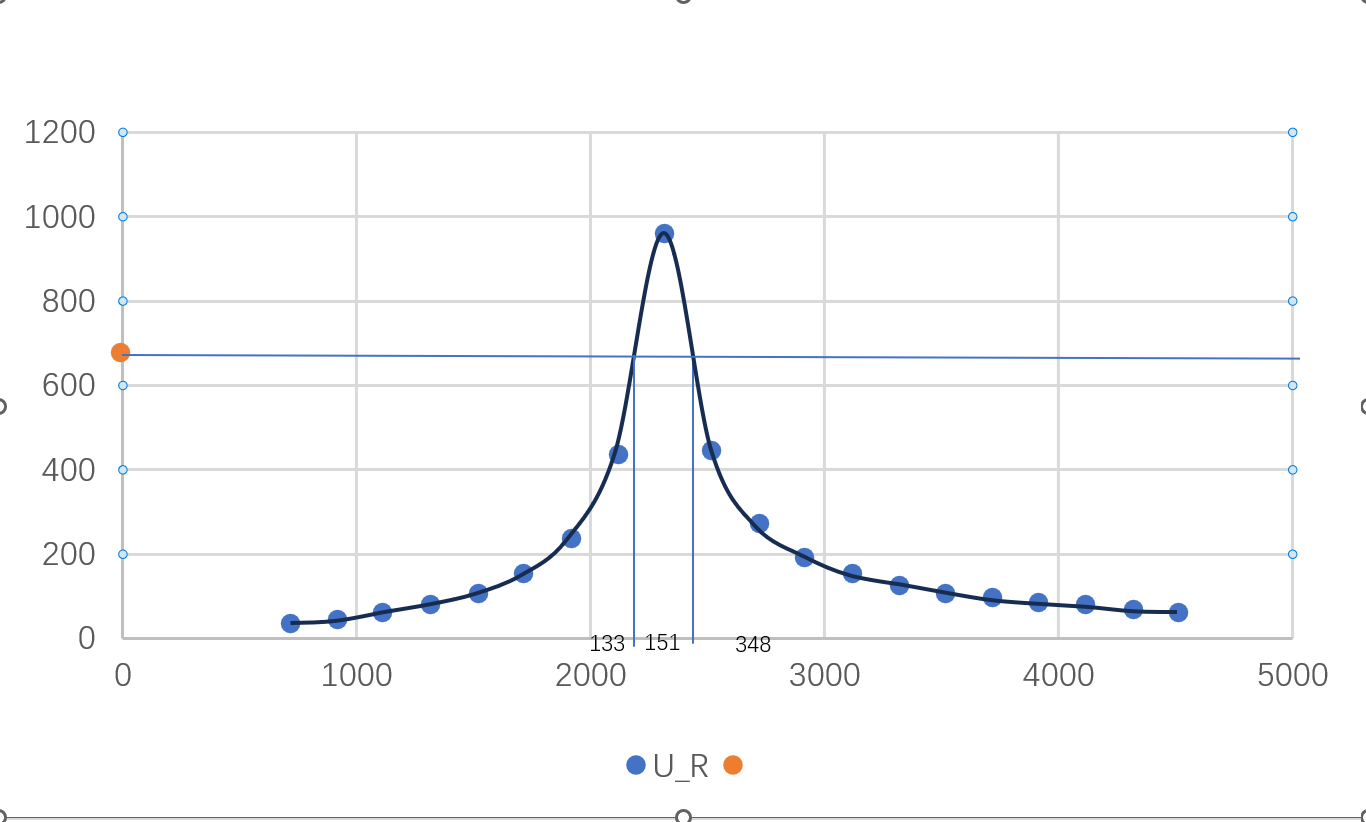
\includegraphics[width=0.3\textwidth,height=0.3\textheight]{f_ur_zuotu.png}
    \caption{$U_{R}-f$图像及处理}
  \end{wrapfigure}

  如图\ref{urf}所示,对图像进行数据处理,确定$\frac{U_{MAX}}{\sqrt{2}}$的水平线,和图形的交点
  作垂线确定$f_{1}\mbox{和}f_{2}$。通过测量和计算可得两者的在x正半轴上的位置分别为
  $f_{1}=2210.443Hz$和$f_{2}=2449.367Hz$。通过公式计算可得
  \begin{equation}
    Q=\frac{f_{0}}{f_{2}-f_{1}}=\frac{2321.521}{2449.367-2210.443}=9.716
  \end{equation}

  通过实验中的测量可以得到实验中电感两端的电压为$344.9mV$,信号源的电压为$41.4mV$,可以得到公式计算可得
  \begin{equation}
    Q=\frac{U_{L}}{U}=\frac{344.9}{41.4}=8.33
  \end{equation}

  实验中测得的数据和理论计算得到的数据的百分差为$14.3\%$,相差较大。
  最终得到的结果误差较大,出现百分差较大的情况,分析误差产生原因:

  1.  测量值可能不够准确,由于器材的误差出现导致实验得到的Q值不够准确。

  2.  理论值可能不够准确,由于理论值通过作图得到,所以最终得到的数值和实际值也存在一定误差

  3.  理论值和实验值都存在误差,导致误差方法出现较大的误差情况出现

\section{思考题}
  \subsection{思考题一}
  RLC电路对不同的频率有不同的阻抗,所以会发生改变。
  \subsection{思考题二}
  它用来描述谐振电路的质量或其谐振能力。 
  Q值越大,通频带宽度就越窄,电路的选择性能越好,抑非能力越强。

  电路品质因数Q值的两种测量方法:
  
  一是根据公式$Q=\frac{UL}{U0}=\frac{UC}{U0}$测定,UC与UL分别为谐振时电容器C和电感线圈L上的电压。

  二是通过测量谐振曲线的通频带宽度$\Delta f=f_{1}-f_{2}$,再根据$Q=\frac{f_{0}}{f_{1}-f_{2}}$求出Q值。
  \subsection{思考题三}
  rlc中l的电阻对谐振曲线的影响是:
  谐振时,对电路总电阻的大小有影响。电阻大,总电阻就大。
  对谐振回路的Q值也有影响,电阻大,Q小。
  对谐振回路的通频带和选择性有影响,电阻大,通频带宽,选择性差。

  测量方法可以通过测量流过电感的电流频率通过$R_{L}=\frac{1}{2\pi * f_{L}}$得到。

\section{实验中个人的思考与感想}
  \subsection{对于实验个人观点}
  实验中使用的器材和书本使用不一样,所用的器材能够通过调节旋钮改变电压表所接接口。实验中可以通过在不同接口处
  连接不同电路部分而可以通过调节旋钮改变实验中电压表所接电路。虽然这样可以方便实验记录,但是实验中的电路连接会导致
  很多问题,导致实验中出现很多未知的问题。而且更多的接口也可能由于接口接触不良等问题导致实验中出现波形难以察觉的问题。

  实验中测量相位差的方式是通过调节示波器上的指针位置读取两指针之间的$\frac{1}{\Delta t}$在进行计算的方法进行实验测试。
  这其中会引入很多不确定度,在调节指针的时候也会出现很大的误差,由于很难调节两指针位置能够恰好满足实验的要求,导致实验
  误差进一步增大。当然这可能和我使用的实验器材有关,似乎隔壁几位的器材由于更为先进所以能直接读出相位差,相较于他们我实验的
  误差应该会更大。
  \subsection{实验中的总结}
  在实验中学习了使用可以调节的元件控制电压表所读对象的方法。实验中电路的连接时实验中较为困难的地方。而实验中
  其余的测量都较为机械化。在测量相位差的时候由于器材的显示进行读数的时候会出现较多误差。而且调节的时候对于
  显示图像也没有放到最大,导致实验中读取的$\frac{1}{\Delta t}$误差较为大。
\end{document}
